\chapter{Analysis}
\label{chap:analysis}

This chapter groups the current analysis paths by acquisition chain. The synchronized beamtime workflow is presently DOGMA based, so the DOGMA section is the scientific core of the chapter. The CAEN, oscilloscope, and DiRICH sections are included for methodological completeness and for future comparative development.

\section{DOGMA analysis}

This section describes the offline methodology applied after the DOGMA edge-stream data have been recorded. It is separated deliberately from the DAQ-systems chapter because the scientific logic of pulse reconstruction, timing-reference control, RF folding, and gamma--neutron separation is not identical to the hardware logic of the front-end electronics.

The active production code is maintained in the repository analysis directory, while exploratory or superseded utilities are moved to the adjacent archive area. Code is edited locally in the mirrored workspace, but authoritative processing is executed remotely on \texttt{padiwa} against the canonical \path{/data6} filesystem. This split preserves version control locally. It also keeps the heavy computation and the large result trees on the storage system for which the workflow was designed.

The present repository begins from DOGMA raw edge files with names such as \texttt{NCAL\_...\_.dld.dat}. Upstream conversion to this edge-stream format is external to the current analysis repository; the workflow described here begins once those files already exist.

For reproducibility, the main storage layout is fixed.

\begin{itemize}
\item Raw DOGMA inputs are stored under \path{/data6/Data/} as \path{*.dld.dat} files.
\item Cleaned pulse tables are stored under \path{/data6/Data/Refined_Data/}.
\item Per-run analysis products are stored under the results root \path{/data6/Dogma_analysis_by_Dachi/Results/}, with one subdirectory per run key.
\item Batch-comparison plots are collected in the \path{Ch02_Position_Comparison/} subtree of that same results root.
\item Archived result sets are kept under \path{Results/Archive/}, with archived cleaned-data directories under \path{/data6/Data/Refined_Data/Archive/}.
\end{itemize}

The analysis uses a compact \emph{run key} derived from the raw filename, for example \path{NCAL_20us_Pos_3.4m_0000}. This run key is then used consistently for refined directories, result directories, summary tables, ROOT outputs, and comparison plots. The convention is operationally important because it allows regenerated products to be compared run by run rather than by full raw filename.

\subsection{Active step map}

Table~\ref{tab:dogma-analysis-step-map} summarizes the currently available production and diagnostic steps in the active DOGMA chain.

\begin{table}[htbp]
\centering
\caption{Current DOGMA cleaned-data workflow and analysis diagnostics.}
\label{tab:dogma-analysis-step-map}
\scriptsize
\setlength{\tabcolsep}{4pt}
\renewcommand{\arraystretch}{1.08}
\begin{tabularx}{\textwidth}{>{\raggedright\arraybackslash}p{1.2cm}>{\raggedright\arraybackslash}p{4.6cm}X}
\toprule
Stage & Main code / primary outputs & Scientific role \\
\midrule
01 & \path{step01_dogma_raw_data_refiner.cpp}, cleaned pulse TSV table & Rise--fall pairing, trigger-window grouping, basic acceptance cuts, and creation of the canonical pulse-level intermediate product. \\
01R & \path{step01_write_cleaned_root_tree.py}, \texttt{CleanedHits} ROOT export & Final reusable pulse-level ROOT representation with timing and RF metadata for downstream studies. \\
02 & \path{step02_*}, all-channel rate summaries and plots & Rate monitoring, run-level sanity checks, and absolute-rate comparisons across channels and runs. \\
03 & \path{step03_*}, trigger-ref and \texttt{ch0}-ref time--ToT products plus whole-run ToT distributions & Time structure, pulse-width distributions, and validation of the timing-reference choice. \\
04 & \path{step04_*}, RF-period scans, folded profiles, folded phase--ToT products, and RF segment tables & Deduction of the RF period, phase folding, and robust handling of within-run RF resets. \\
05 & \path{step05_estimate_gamma_neutron_background.py}, sideband background summaries & First-pass local background estimates in phase--ToT space. \\
06 & \path{step06_quantify_gamma_neutron_components.py}, ROI overlays, projections, and component tables & Quantification of prompt-gamma and constrained fast-neutron candidate regions with explicit overlap flags. \\
07 & \path{step07_phase_rate_slice_diagnostics.py}, one-period phase-rate slices and excess intervals & One-dimensional delayed-excess diagnostics before finalizing two-dimensional selections. \\
08 & \path{step08_fit_gamma_tot_peak.py}, gamma-ToT peak-fit tables and figures & Run-by-run centering of the compact prompt-gamma ToT feature in a narrow fit interval. \\
09 & \path{step09_gamma_window_sensitivity.py}, width-sensitivity summaries & Systematic study of prompt-gamma reference stability under different centered ToT-gate widths. \\
10 & \path{step10_gamma_reference_cfd.py}, reference-comparison diagnostics & Comparison of local-fit, raw-maximum, and CFD-style prompt-gamma reference definitions. \\
Batch & \path{run_all_cleaned_analysis_chain.py}, synchronized per-run result trees & Reproducible remote orchestration of the cleaned-data production chain. \\
\bottomrule
\end{tabularx}
\end{table}

The numerically heavy transformations remain in compiled C++ code, whereas Python is used mainly for orchestration, file management, bookkeeping, and rendering. This separation is deliberate: the workflow needs compiled performance for long runs, but it also needs enough scripting flexibility to regenerate summaries, diagnostics, and comparison plots without rewriting the analyzers themselves.

\subsection{Pulse reconstruction and timing observables}

\subsubsection{Pulse cleaning as the canonical intermediate}

The first production step is implemented in \path{step01_dogma_raw_data_refiner.cpp} and driven by \path{step01_run_dogma_raw_data_refiner.py}. Its purpose is to convert raw edge information into a cleaned pulse table. Conceptually, the raw DOGMA file contains edge-level information, whereas the later physics studies require pulse-level quantities. The cleaner therefore groups edges into trigger windows, matches rising and falling edges to form pulses with well-defined rise time, fall time, and time-over-threshold (ToT), rejects isolated or inconsistent edges, applies configurable acceptance limits, and writes run-level summary files so that anomalies remain auditable.

This step is also the natural place to guard against global-time discontinuities. The refined pulse table is therefore treated as the canonical reusable intermediate product: once it exists and has passed sanity checks, most later analysis stages can be regenerated without rereading the original raw edge file. The final ROOT writer, \path{step01_write_cleaned_root_tree.py}, consumes the same cleaned pulse table together with the RF-segmentation metadata and writes the split \texttt{CleanedHits} export used for later reuse.

\subsubsection{Rate, ToT, and timing-reference products}

After pulse cleaning, \path{step02_*} writes cleaned all-channel rate products, while \path{step03_*} writes trigger-referenced and \texttt{ch0}-referenced time--ToT products together with per-channel ToT distributions. These outputs are scientifically useful for two reasons. First, they verify that the cleaned pulse table is populated by accepted pulse candidates rather than by unmatched edges. Second, they expose the prompt-like pulse-width feature that later becomes the anchor for the gamma reference.

Two timing reference frames are used throughout the cleaned-data chain.

\begin{enumerate}
\item \textbf{Trigger-referenced time}, where pulse times are measured relative to the hardware trigger.
\item \textbf{Channel-0-referenced time}, where pulse times are measured relative to the accepted reference pulse on channel~0 within the same trigger window.
\end{enumerate}

The \texttt{ch0} reference is physically important because channel~0 carries the discriminated timing signal derived from the machine RF chain. In the current implementation, a \texttt{ch0} candidate is accepted only if its rise time and ToT fall inside a predefined validity window. If several valid candidates are present, the first valid one is selected, and companion statistics files are written so that this choice can be audited later. For a non-reference channel, the key timing quantity is therefore
\begin{equation}
t_{\mathrm{ch0\,ref}} = t_{\mathrm{rise}}^{(\mathrm{ch})} - t_{\mathrm{rise}}^{(\mathrm{ch0})}.
\end{equation}

Figure~\ref{fig:dogma-ch02-tot-distribution} shows a representative whole-run channel-2 ToT spectrum from the cleaned pulse table. The narrow peak near \SI{13.5}{ns} is the compact prompt-like feature later isolated by the step-08 fit, while the broad lower-ToT and higher-ToT structures demonstrate why a narrow, dynamically centered prompt-gamma gate is preferable to a fixed hard-coded ToT interval.

\begin{figure}[htbp]
\centering
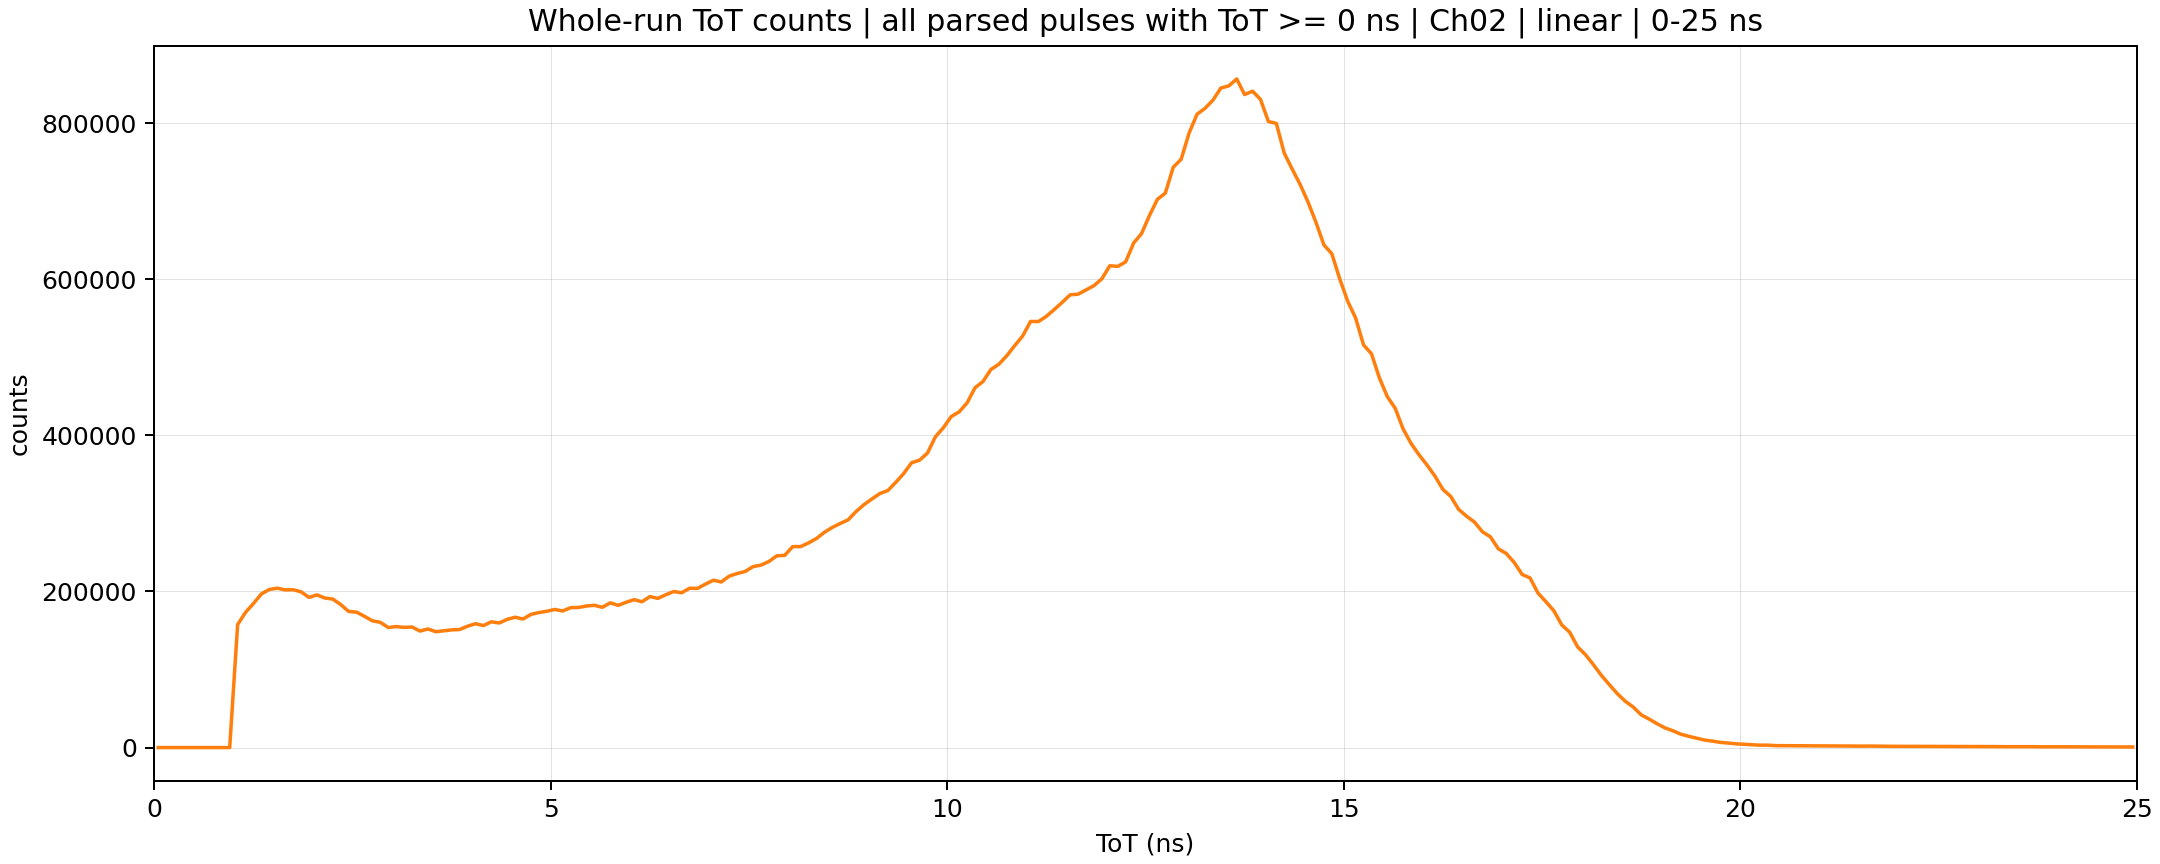
\includegraphics[width=0.88\textwidth]{../../Dogma_Analysis/Results/Position Runs/TOT_Distributions_AllRuns/NCAL_20us_Pos_5m_0000_ch02_tot_distrib.png}
\caption{Representative whole-run cleaned channel-2 ToT distribution for the \SI{5.0}{m} position run. The spectrum is built from accepted pulses after edge pairing and cleaning. The sharp feature near \SI{13.5}{ns} is the compact prompt-like ToT component later used for run-by-run gamma-gate centering, whereas the broad surrounding structure motivates a two-stage prompt-reference treatment rather than a fixed global cut.}
\label{fig:dogma-ch02-tot-distribution}
\end{figure}

\subsubsection{RF period deduction and folded observables}

\paragraph{Measured millisecond trigger envelope.}
\phantomsection
\label{sec:dogma-trigger-envelope}
The fast RF period must be distinguished from a slower modulation of the recorded trigger population. A cyclotron-control-room oscilloscope photograph supplied during the timing investigation shows an approximately \SI{1}{ms} per division timebase, a pattern repeating approximately every \SI{6.6}{ms} to \SI{6.7}{ms}, and a short interval of about \SI{1.2}{ms} to \SI{1.4}{ms} associated with bursts on the second trace (Figure~\ref{fig:cyclotron-control-envelope}). This is consistent with the operational recollection of approximately \SI{150}{Hz} modulation and approximately 20\% active duty. The photograph motivates that hypothesis, but does not by itself identify the scope-channel wiring, active polarity, or an exact beam-current duty cycle.

\begin{figure}[htbp]
\centering
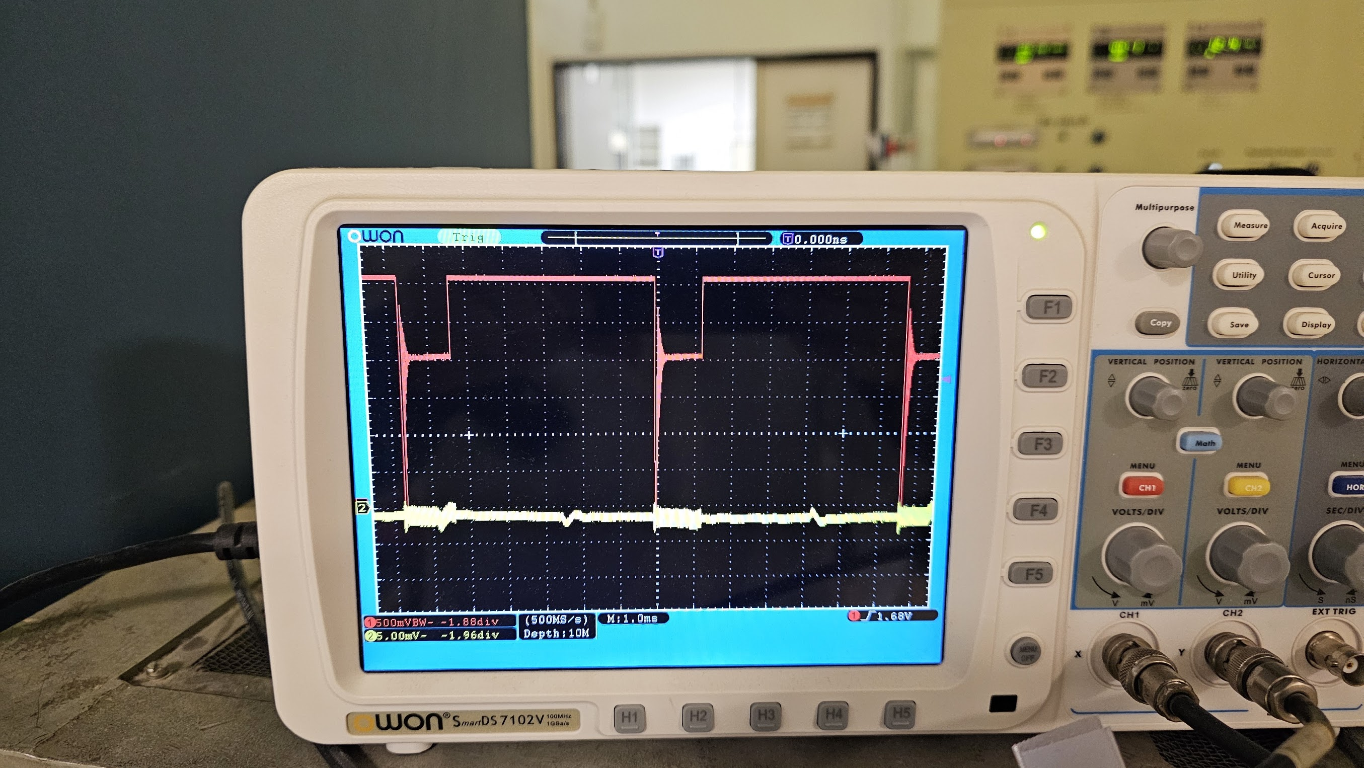
\includegraphics[width=0.92\textwidth]{figures/cyclotron_control_room_rf_envelope.png}
\caption{Cyclotron-control-room oscilloscope photograph supplied as timing context. The short interval occupies approximately one fifth of the repeating millisecond-scale pattern, and the yellow bursts appear associated with the low portion of the pink trace. Individual RF cycles are not resolved at this timebase. Trace identities and the hardware gating mechanism are not inferred from the photograph alone.}
\label{fig:cyclotron-control-envelope}
\end{figure}

The hypothesis was tested independently of detector-pulse and timing-reference cuts using every original \texttt{TDC\_001049} trigger-window header in a fresh decode of the canonical \SI{5.0}{m} \texttt{\_0000} recording. All 10,516,211 timestamps were retained, including windows without a passing cleaned \texttt{ch0} reference. The original \texttt{GlobalTriggerTime} values were mapped to their native \SI{5}{ns} integer-counter lattice before differences were formed. Their absolute DAQ-time range is \SI{902.178410820}{s} to \SI{2952.996736650}{s}, spanning \SI{2050.818325830}{s}; these are DAQ counter times, not UTC. Figure~\ref{fig:dogma-absolute-trigger-envelope} shows the full distribution and unfiltered early, middle, and late examples.

\begin{figure}[p]
\centering
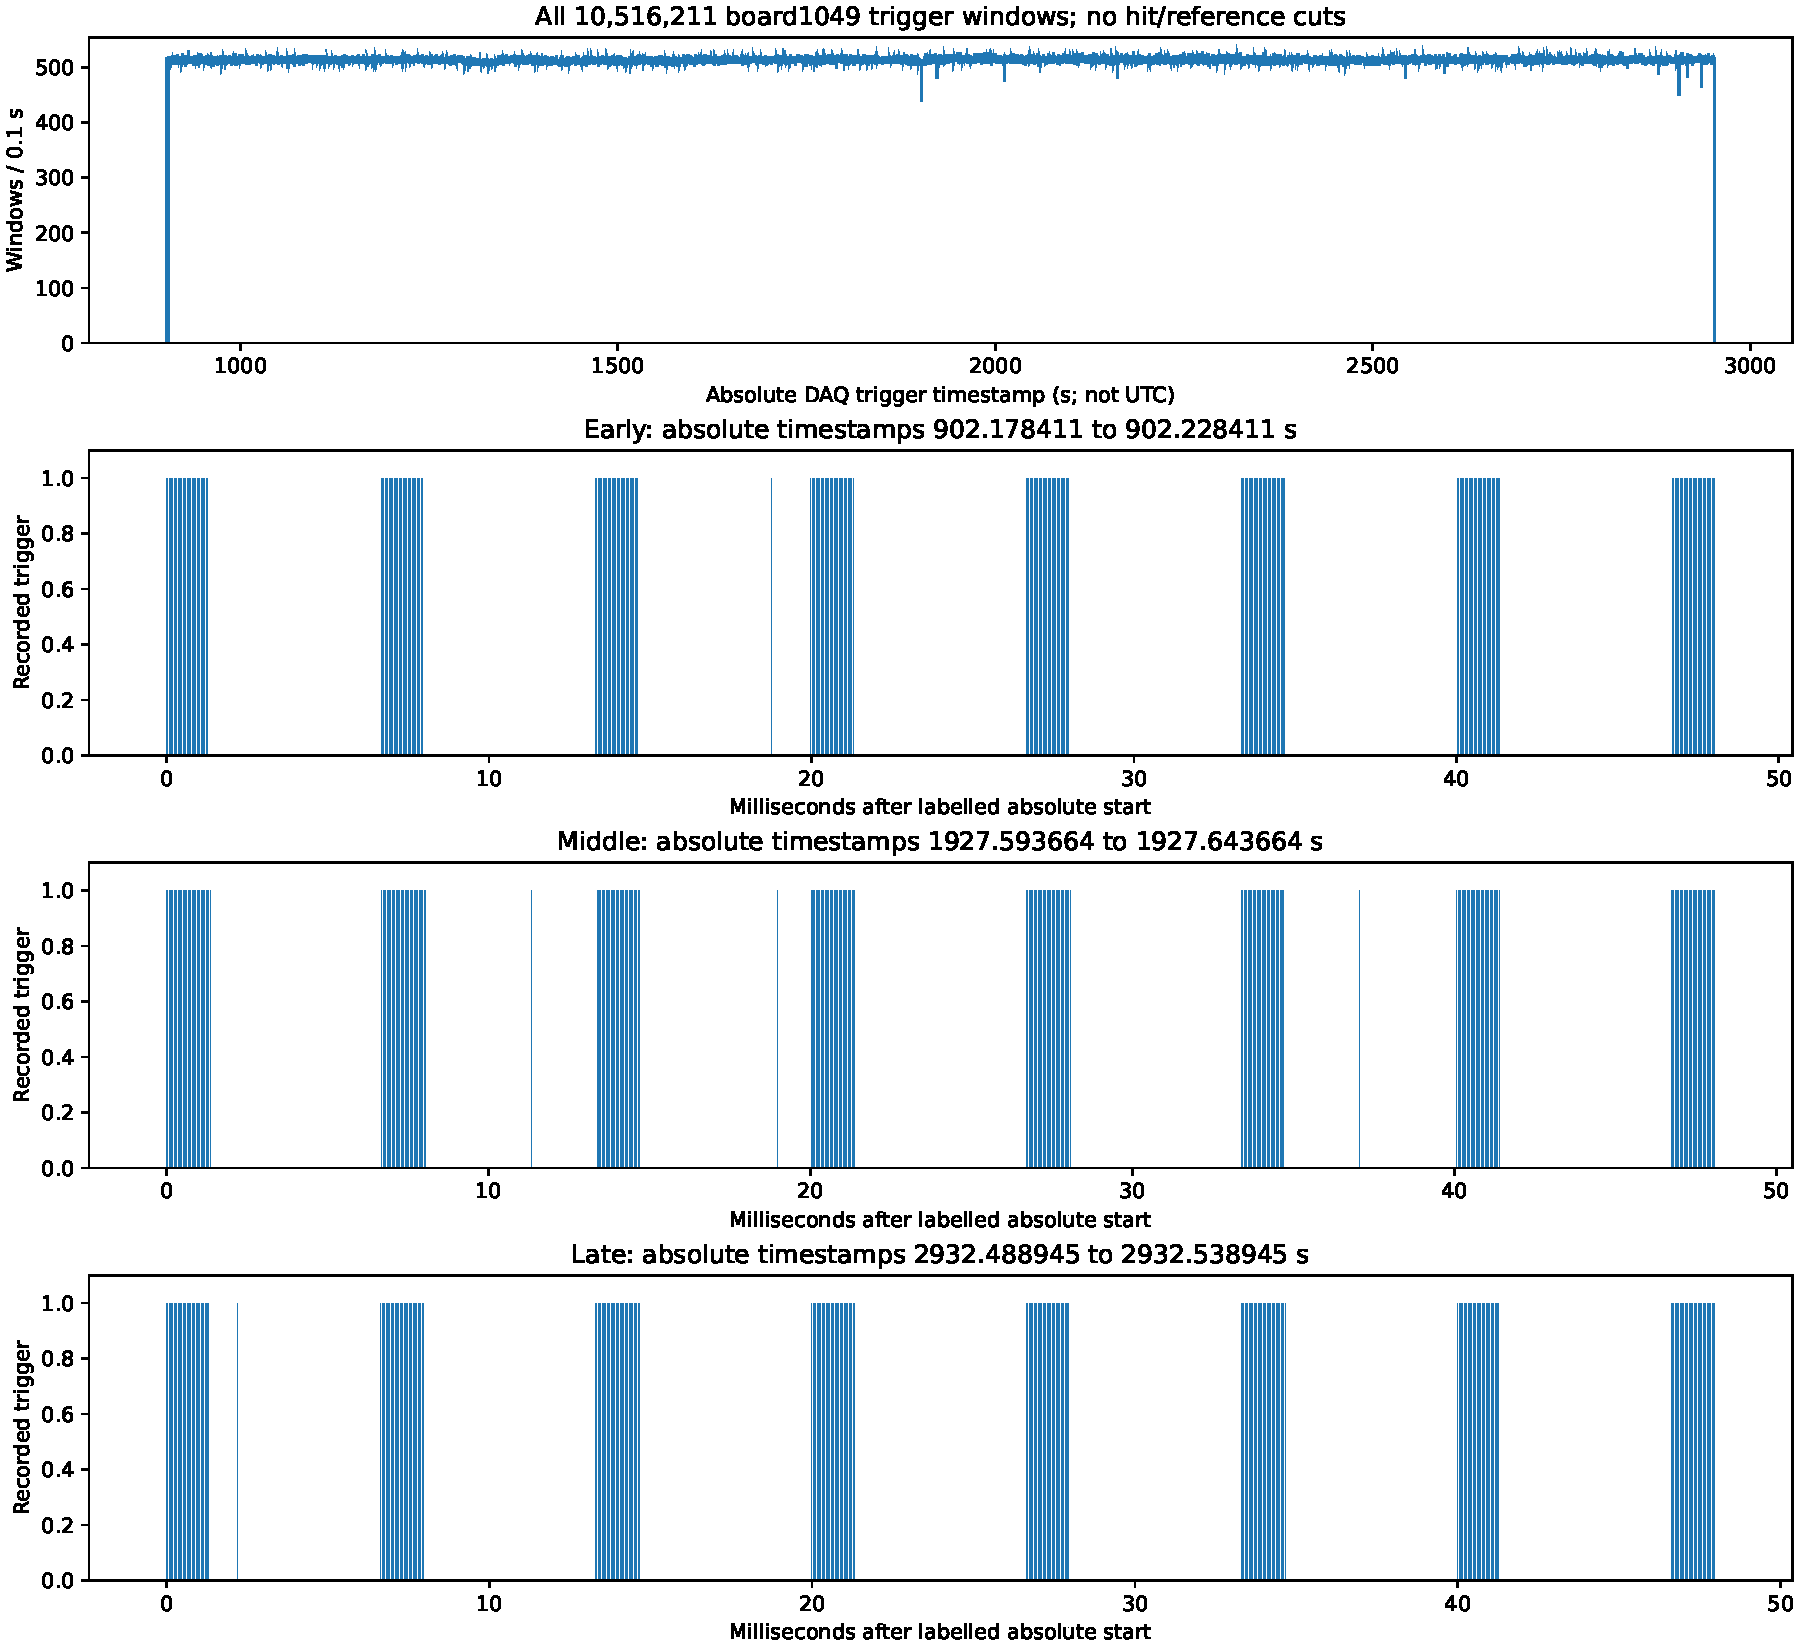
\includegraphics[width=\textwidth,height=0.78\textheight,keepaspectratio]{../../Dogma_Analysis/Results/Position Runs/Zebra Period Finder/NCAL_20us_Pos_5m_0000/step00 - Decode/Trigger timing/absolute_trigger_timestamp_distribution.pdf}
\caption{Absolute DAQ trigger-window timestamp distribution for all 10,516,211 board1049 windows, without edge, ToT, \texttt{ch0}-reference, or clock-support cuts. The upper panel uses \SI{0.1}{s} bins over the recording. The lower panels retain every trigger in three \SI{50}{ms} intervals identified by their absolute starting timestamps. Dense bursts approximately \SI{1.3}{ms} wide repeat on a \SI{6.67}{ms} timescale; sparse inter-burst triggers are also visible.}
\label{fig:dogma-absolute-trigger-envelope}
\end{figure}

For envelope measurement only, consecutive timestamps separated by at most \SI{0.2}{ms} were grouped and groups with at least eight triggers were labelled dense; sparse groups were not removed from the absolute distribution or accounting. This identifies 307,491 dense bursts containing 10,458,943 windows, or approximately 99.455\% of the recording, alongside 57,268 sparse-group windows. Dense bursts typically contain 33--35 triggers, with median within-group spacing \SI{39.780}{\micro\second}. Their median start-to-start spacing is \SI{6.665070}{ms}. Regression in blocks of at most 256 burst starts, without assigning cycle counts across nonregular gaps, gives an aggregate repetition period of approximately \SI{6.665156}{ms}, or \SI{150.034}{Hz}. No \SI{150}{Hz} template or 20\% duty selection was imposed.

The median observed first-to-last trigger span is \SI{1.312830}{ms}. Since those first and last triggers need not coincide with the envelope boundaries, a recorded-trigger occupancy proxy is defined by
\begin{equation}
d_{\mathrm{trig}} =
\frac{t_{\mathrm{last}}-t_{\mathrm{first}}+\widetilde{\Delta t}_{\mathrm{within}}}
     {t_{\mathrm{first,next}}-t_{\mathrm{first}}},
\end{equation}
where $\widetilde{\Delta t}_{\mathrm{within}}$ is the median within-group trigger spacing. This gives a median proxy of 20.29\%, with a central 68\% range of 19.78--20.81\%; the median corrected span is \SI{1.352610}{ms}. The one-spacing endpoint convention is about 0.6 percentage point on this cycle, so these values are not an exact independently measured RF-on gate or beam-current duty. The median separation from the last trigger of a dense burst to the first of the next is \SI{5.352940}{ms}; sparse triggers can occur inside that separation.

The feature persists throughout ten equal-duration recording segments, whose fitted repetition frequencies range from \SI{149.817}{Hz} to \SI{150.234}{Hz} and whose median duty proxies range from 20.267\% to 20.316\%. Grouping thresholds from \SI{0.1}{ms} to \SI{1.0}{ms} reproduce the same dense-burst count and give frequencies approximately \SI{150.034}{Hz} to \SI{150.068}{Hz}; density classifications were also varied. These spreads describe sensitivity and observed variation, not statistical confidence intervals. All absolute histogram bins were independently checked with integer counters, and 10,518 sampled original timestamp strings were independently checked by decimal arithmetic.

\textbf{The approximately \SI{150}{Hz}, approximately 20\% recorded-trigger envelope is therefore an established feature of this recording, consistent with the scope image.} The physical interpretation as modulation of the RF-derived timing chain is supported, but timestamps alone do not distinguish RF-amplitude suppression, discriminator threshold effects, trigger gating, or actual carrier interruption. Sparse triggers are explicitly retained, and a separate \SI{1.280333970}{s} inter-trigger gap remains outside the ordinary modulation explanation. Other runs require their own checks.

Consequently, ordinary inter-burst gaps must not automatically be labelled data loss, corrupted time, machine restarts, or RF phase resets. Nor should otherwise valid detector hits be discarded merely because a symmetric local-period estimator lacks neighbours at a natural burst boundary. The earlier gap-aware ch0 diagnostic imposed such a support selection and is a selected-subset diagnostic, not a matched-population alternative to the original ch2 estimator. Period-estimator comparisons must use the same cleaned, referenced detector hits and explicitly state any constant-period or cross-burst phase-continuity assumptions. This timestamp investigation changes no existing pulse-selection or folded-histogram product.

The RF-folding step, implemented in \path{step04_*}, deduces a best RF period $P$ and a phase origin $\phi_0$ from a score channel, which is currently channel~2 by default. The folded phase is written using the \texttt{ch0}-referenced rise time,
\begin{equation}
\phi = \operatorname{mod}\!\left( t_{\mathrm{ch0\,ref}} - \phi_0,\; P \right).
\end{equation}
This distinction is physically essential: trigger-referenced times and channel-0-referenced times are both useful, but the folded RF products are intended to characterize detector timing relative to the RF reference, so the meaningful phase coordinate is the channel-0-referenced one.

The current robust version of the workflow also supports within-run RF segmentation. If the cyclotron is stopped and restarted during one run, one global phase origin is no longer sufficient. The patched step-04 analyzer therefore searches time-ordered score pulses for persistent phase jumps, writes a phase-segment table, and passes that segmentation to the final ROOT writer through the \texttt{rf\_segment\_id} branch. In this way, a restart no longer forces the entire run to share one RF phase origin.

\subsection{Robustness controls and diagnosed failure modes}

Several conceptually different problems were encountered during commissioning, and they materially shaped the current workflow.

\paragraph{Edge pairing and \texttt{ch0} ambiguity.}
The first class of questions concerned whether the cleaner was pairing edges in a physically sensible way and how robust the \texttt{ch0} reference selection remained when multiple candidates appeared in the same trigger window. The practical response was to treat the pulse cleaner as the authoritative rise--fall pairing stage and to extend the runners so that odd-\texttt{ch0} statistics and sample files are written explicitly. Ambiguities can therefore be inspected directly instead of being inferred indirectly from final plots.

\paragraph{RF phase--ToT combs.}
The folded RF phase-versus-ToT plots showed persistent negative-slope diagonal structures. The decisive diagnostic, using \path{phi_star_artifact_diagnostic.py} together with direct comparisons between pre-fold and post-fold outputs, showed that these structures are not introduced by the rendering or folding stage itself. The software can sharpen them, but it is not their primary origin. The working interpretation is therefore that the reference or signal chain contains preferred timing families that become visible once the data are folded.

\paragraph{Reference-chain interpretation.}
Once the software-artifact hypothesis became unlikely, attention shifted to the hardware timing chain. In particular, the RF sine is converted to logic through a discriminator path, so threshold-crossing families in that chain remain a plausible source of structured timing bunching. In this interpretation, the analysis code is correctly exposing a property of the timing-reference chain rather than inventing one.

\paragraph{Reproducibility of long reruns.}
For the large runs, the workflow cost is not dominated solely by the initial cleaner. RF folding and final ROOT export can each consume substantial wall time. This motivated two policies that remain central to the present chain: the cleaned pulse table is treated as the stable handoff between raw edge decoding and higher-level timing analysis, and regenerated remote products are archived run-key by run-key rather than overwritten without trace.

\subsection{Gamma--neutron component studies}

The folded RF phase-versus-ToT plots are useful for developing gamma--neutron separation strategies, but they should not be interpreted as direct particle-identification maps without a background model. The radiation field seen by NCAL is mixed. It can contain prompt gammas from source-station materials, secondary capture gammas, room and shielding backgrounds, scattered neutrons, continuum neutrons from the beryllium target, random coincidences, electronic pickup, and residual timing-chain artifacts. For this reason, a compact region in phase--ToT space should be called gamma-like or neutron-like only after the non-beam and off-region contributions have been characterized.

The working strategy is hierarchical. First, beam-off, blocked-aperture, or sideband regions should be used where available to estimate components that are not correlated with prompt beam timing. Second, cleanly separated regions of the position scan can be used to define empirical gamma-like and neutron-like templates. Third, regions where the two populations overlap should be treated statistically rather than by hard event labels. In an overlapped phase--ToT region, the observed density is represented schematically as
\begin{equation}
N(\phi,\mathrm{ToT}) = A_{\gamma} G(\phi,\mathrm{ToT}) + A_{n} N_{n}(\phi,\mathrm{ToT}) + B(\phi,\mathrm{ToT}),
\end{equation}
where $G$ is the prompt-gamma-like template, $N_n$ is the neutron-like template, and $B$ is the residual background model. Under such conditions, individual hits should not be assigned uniquely to gamma or neutron populations using phase and ToT alone; they should instead receive probabilistic weights or appear only in fitted yield estimates with explicit overlap uncertainty.

An analytical time-of-flight reference is also needed to show why the position scan is expected to help. For a detector-face distance $d$, the prompt-gamma time is
\begin{equation}
t_{\gamma}(d) = \frac{d}{c},
\end{equation}
while a neutron with kinetic energy $E_n$ has
\begin{equation}
\beta_n(E_n) = \sqrt{1 - \left(1 + \frac{E_n}{m_n c^2}\right)^{-2}},
\qquad
t_n(d,E_n) = \frac{d}{\beta_n c}.
\end{equation}
The reference separation is therefore
\begin{equation}
\Delta t(d,E_n) = t_n(d,E_n) - t_{\gamma}(d).
\end{equation}
For the present campaign, \SI{30}{MeV} is used as the main reference energy because the measured forward proton-on-beryllium spectra at NPI show prominent high-energy structure near \SIrange{30}{32}{MeV} and extend to about \SI{33}{MeV} for the thick-target configuration \citep{Majerle2023PBeGenerator,Ansorge2025CollimatedBeams}. This should be understood as a representative fast-neutron reference curve, not as a monoenergetic source model.

Figure~\ref{fig:gamma-neutron-tof-reference-positions} shows the resulting prompt-gamma and fast-neutron time-of-flight curves for the position-scan distances. The \SI{30}{MeV} reference gives separations of about \SI{28.5}{ns}, \SI{34.6}{ns}, \SI{40.7}{ns}, \SI{50.9}{ns}, \SI{59.0}{ns}, and \SI{67.2}{ns} at \SIlist{2.8;3.4;4.0;5.0;5.8;6.6}{m}, respectively. Since slower continuum neutrons arrive later, this reference marks the early fast-neutron scale rather than the full neutron timing envelope.

\begin{figure}[htbp]
\centering
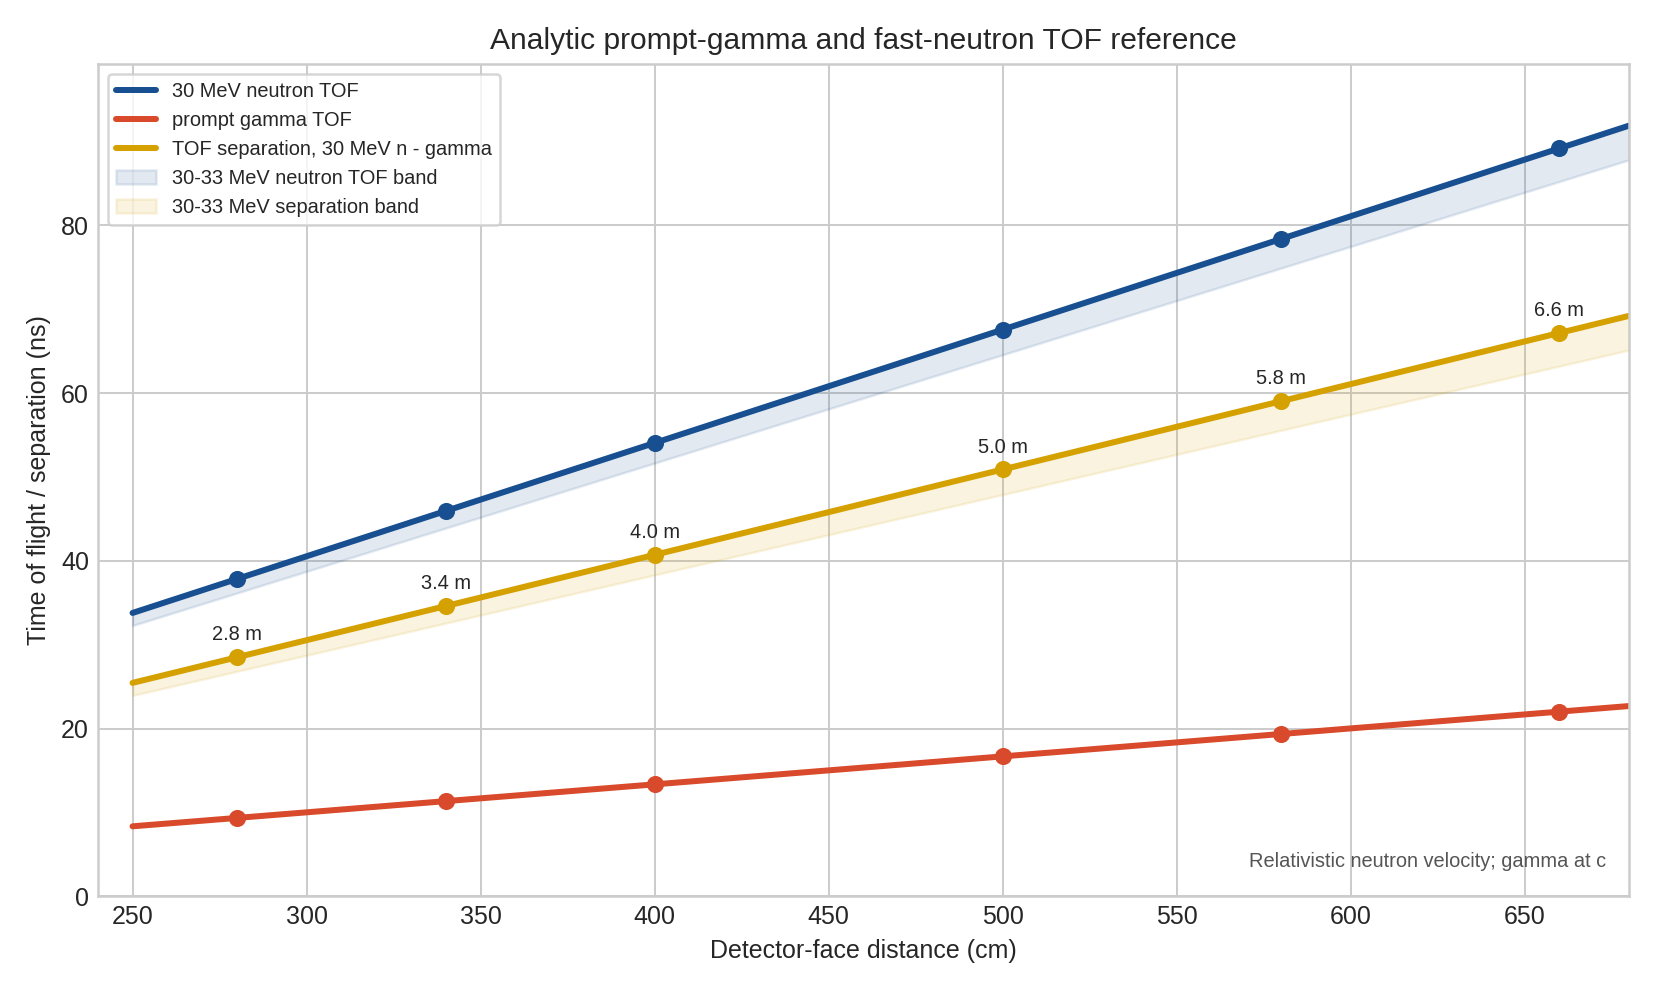
\includegraphics[width=0.92\textwidth]{figures/Gamma_Neutron_deltaTOF_30MeV_reference_positions.png}
\caption{Analytical prompt-gamma and fast-neutron time-of-flight reference for the NCAL position scan. The central neutron curve uses \SI{30}{MeV}; the shaded band indicates the small change between \SI{30}{MeV} and \SI{33}{MeV}. The \SI{30}{MeV} choice is a representative fast-neutron reference within the high-energy part of the \SI{35}{MeV} proton-on-beryllium spectrum, not a monoenergetic source assumption.}
\label{fig:gamma-neutron-tof-reference-positions}
\end{figure}

The qualitative motivation for this treatment is visible directly in the folded RF phase-versus-ToT products. Figure~\ref{fig:position-scan-phase-tot-panel} collects representative channel-2 maps from the completed position-scan runs, with detector-face distance stated explicitly above each panel. The compact prompt-like island remains narrow in phase and ToT, whereas the broader neutron-dominated structure changes its relative timing as the detector distance is varied. The figure is included to show the observable space in which later component modeling must operate; the different panels should not be read as an absolute yield comparison because the displayed density scales are plot-level renderings.

\begin{landscape}
\begin{figure}[p]
\centering
\begin{minipage}{0.32\linewidth}
\centering
{\small\bfseries Detector face: \SI{2.8}{m}}\\[0.25em]
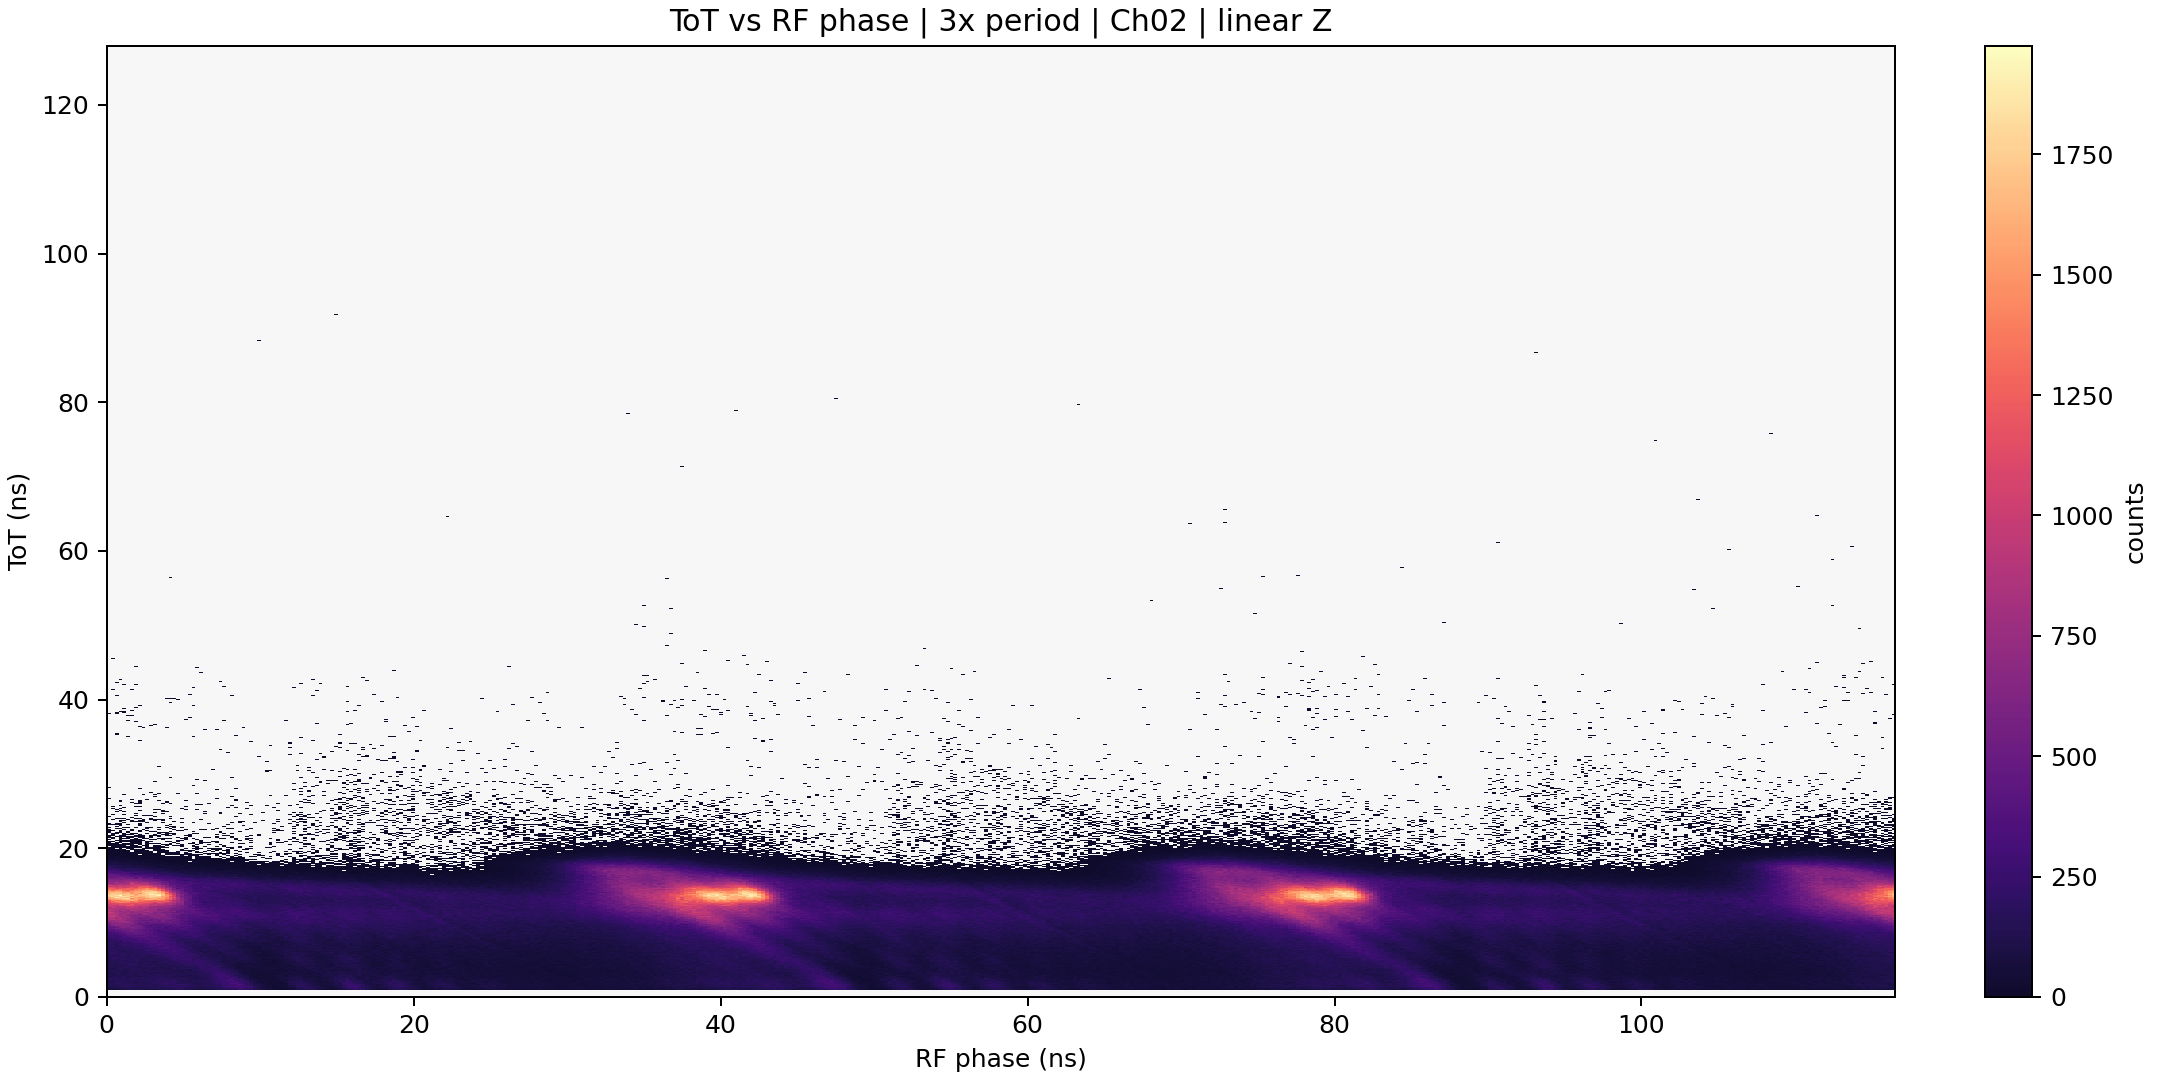
\includegraphics[width=\linewidth]{figures/phase_tot_position_scan/pos_2p8m_ch02_rf_phase_3x_vs_tot.png}
\end{minipage}\hfill
\begin{minipage}{0.32\linewidth}
\centering
{\small\bfseries Detector face: \SI{3.4}{m}}\\[0.25em]
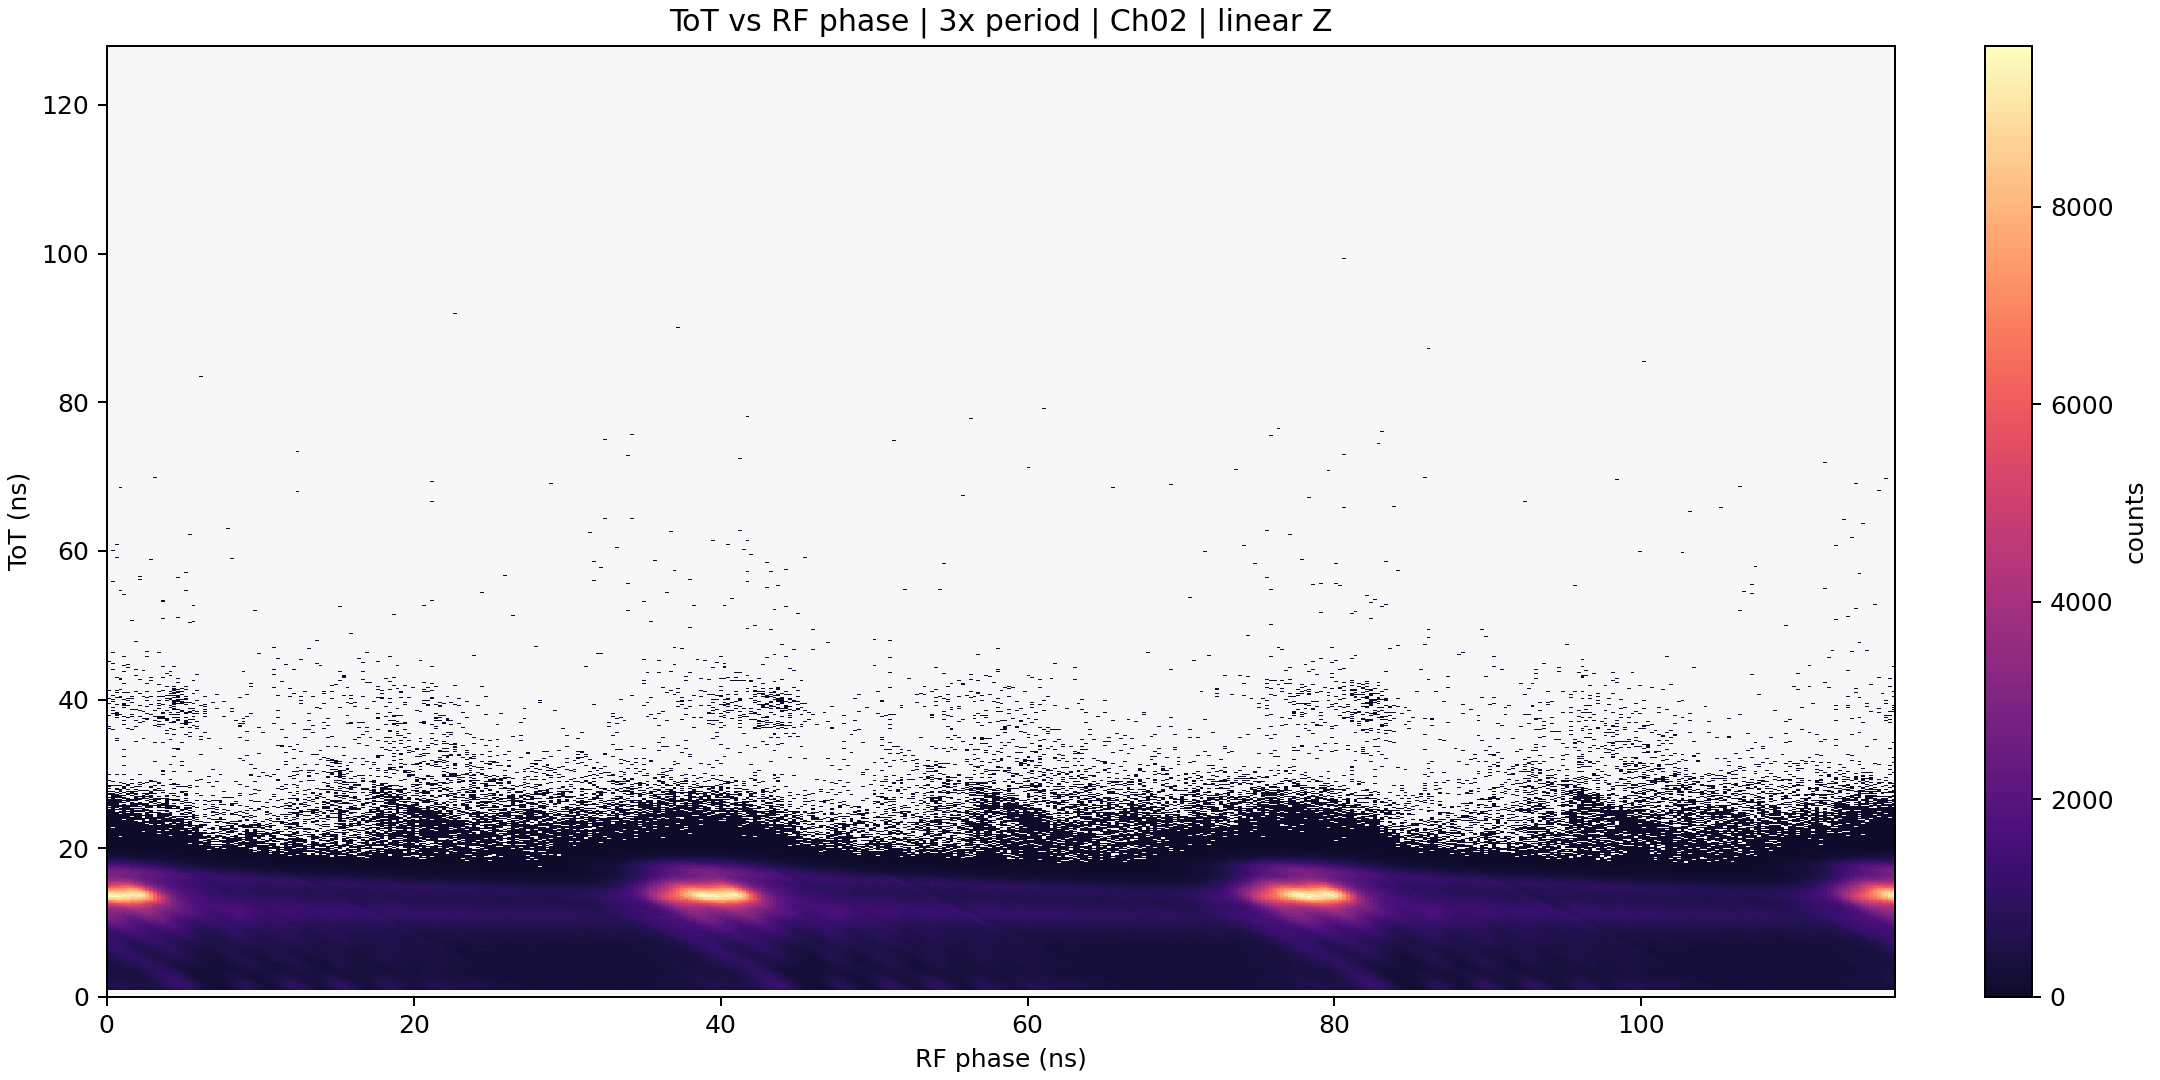
\includegraphics[width=\linewidth]{figures/phase_tot_position_scan/pos_3p4m_ch02_rf_phase_3x_vs_tot.png}
\end{minipage}\hfill
\begin{minipage}{0.32\linewidth}
\centering
{\small\bfseries Detector face: \SI{4.0}{m}}\\[0.25em]
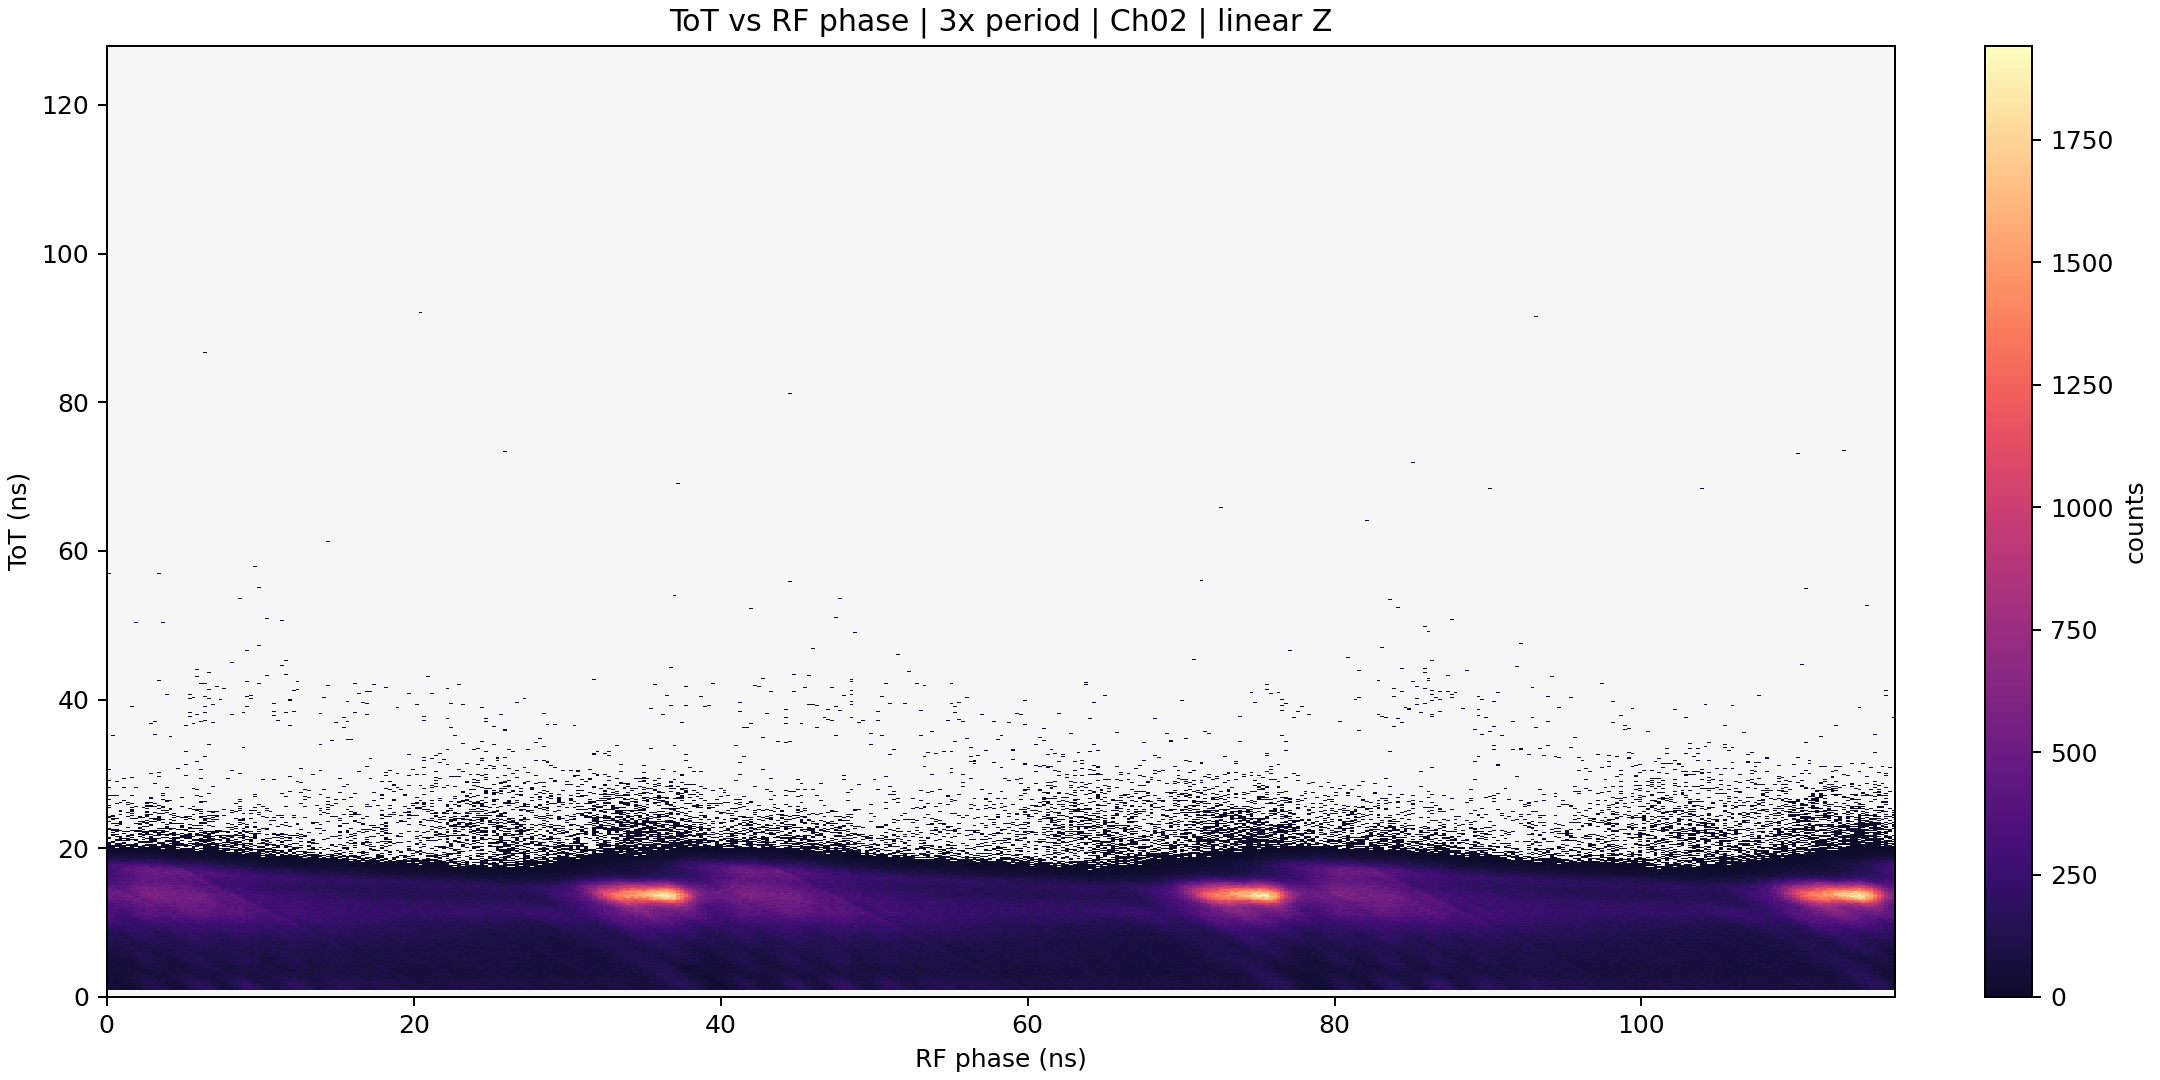
\includegraphics[width=\linewidth]{figures/phase_tot_position_scan/pos_4p0m_ch02_rf_phase_3x_vs_tot.png}
\end{minipage}

\vspace{0.5cm}

\begin{minipage}{0.32\linewidth}
\centering
{\small\bfseries Detector face: \SI{5.0}{m}}\\[0.25em]
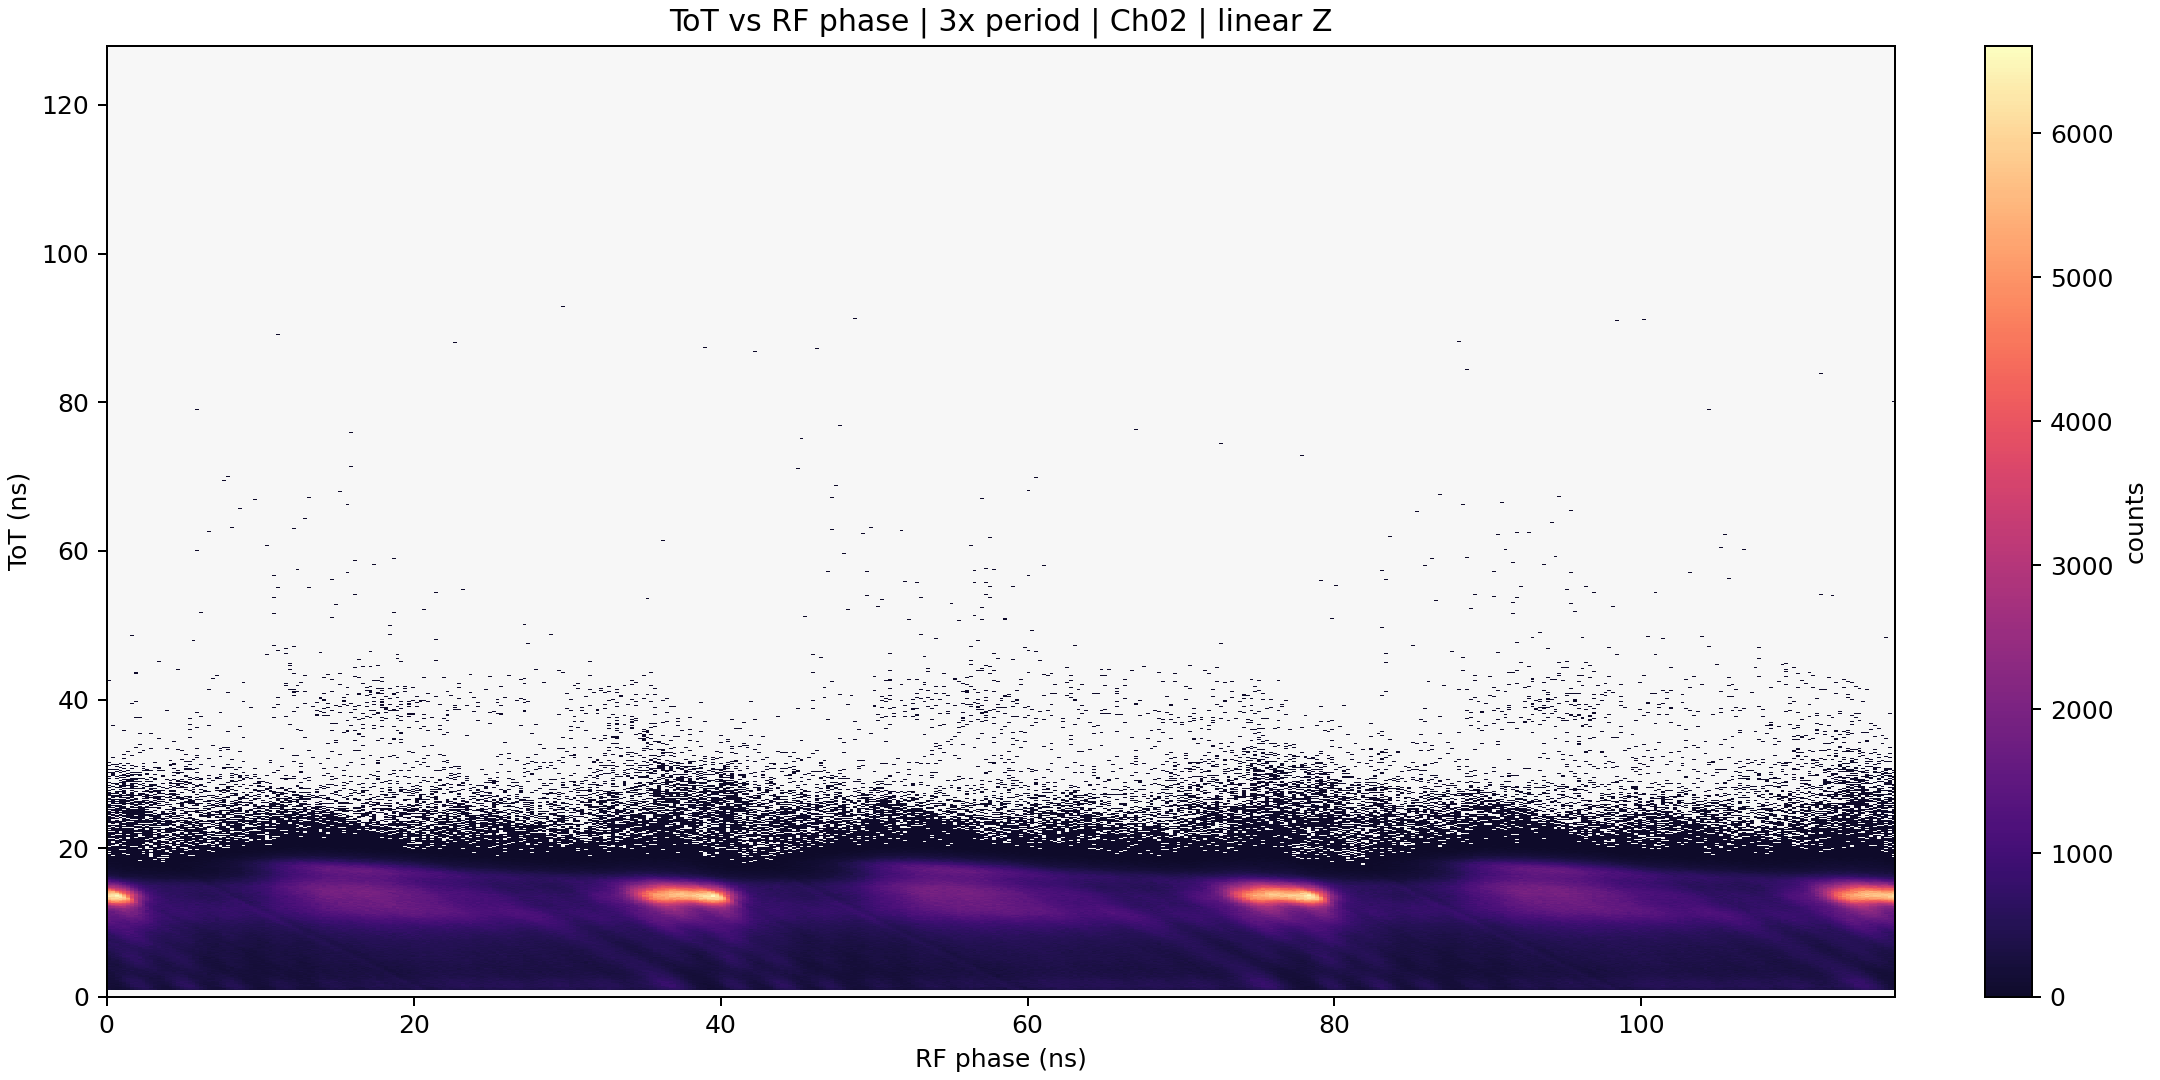
\includegraphics[width=\linewidth]{figures/phase_tot_position_scan/pos_5p0m_ch02_rf_phase_3x_vs_tot.png}
\end{minipage}\hfill
\begin{minipage}{0.32\linewidth}
\centering
{\small\bfseries Detector face: \SI{5.8}{m}}\\[0.25em]
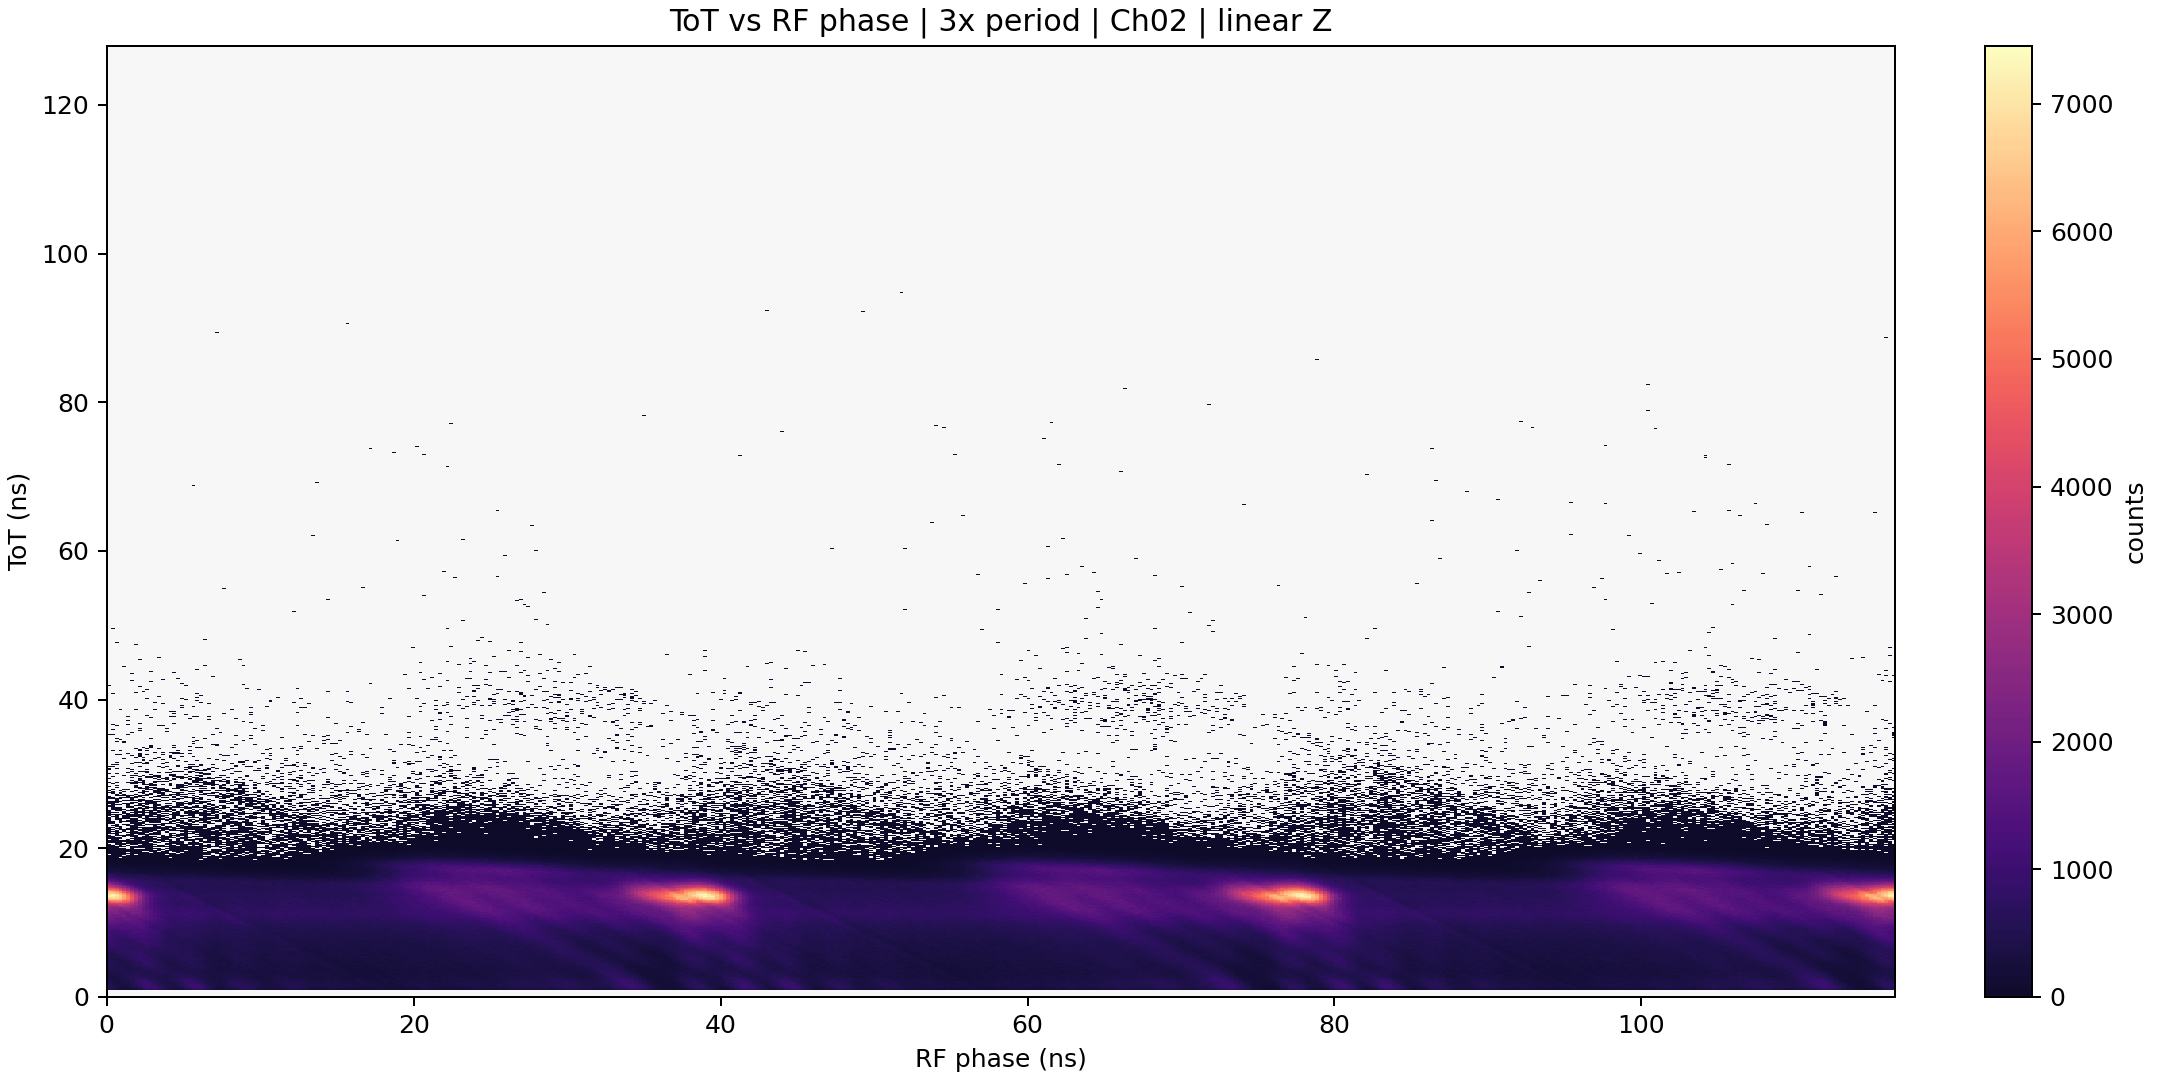
\includegraphics[width=\linewidth]{figures/phase_tot_position_scan/pos_5p8m_ch02_rf_phase_3x_vs_tot.png}
\end{minipage}\hfill
\begin{minipage}{0.32\linewidth}
\centering
{\small\bfseries Detector face: \SI{6.6}{m}}\\[0.25em]
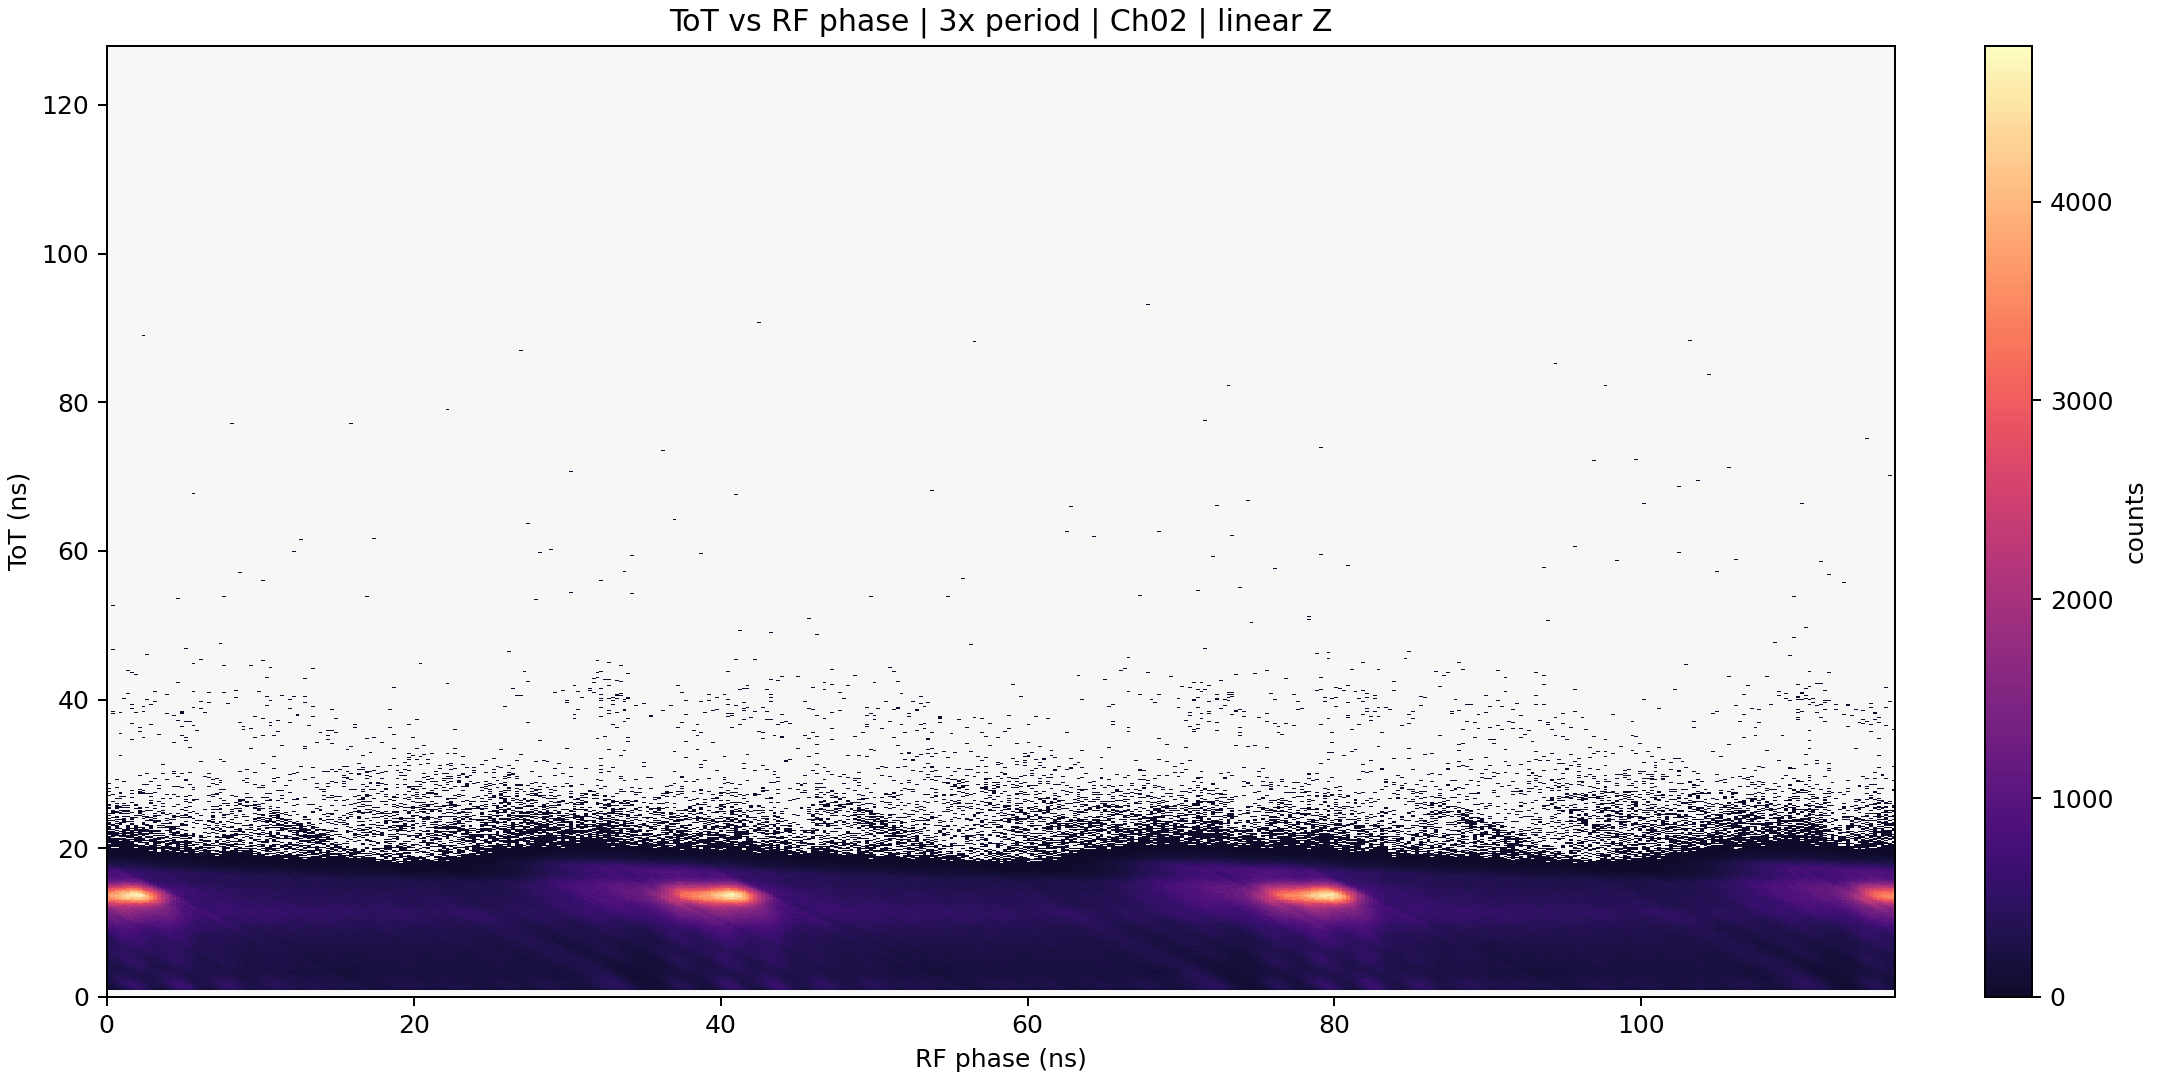
\includegraphics[width=\linewidth]{figures/phase_tot_position_scan/pos_6p6m_ch02_rf_phase_3x_vs_tot.png}
\end{minipage}
\caption{Position-scan view of NCAL channel~2 in folded RF phase and time-over-threshold. Each panel shows the same observable space over three RF periods for a different detector-face distance. At some positions the compact prompt-like island is visibly separated from the broader neutron-dominated distribution, whereas in overlap regions the event content must be treated as a statistical mixture rather than by unique hit-by-hit labels. The \SI{4.0}{m} panel uses the completed \texttt{NCAL\_20us\_Pos\_4m\_0001} run.}
\label{fig:position-scan-phase-tot-panel}
\end{figure}
\end{landscape}

The first-pass background estimator, \path{step05_estimate_gamma_neutron_background.py}, uses local sidebands to protect the prompt-gamma and neutron-candidate regions against obvious contamination. The more developed \path{step06_quantify_gamma_neutron_components.py} then measures prompt-gamma centroids and widths independently for each run, draws the nominal \SI{30}{MeV} neutron guide, defines protected background sidebands, and reports background-subtracted prompt-gamma and constrained fast-neutron candidate rates. The direct neutron quantity produced by step~06 is intentionally narrow in phase and ToT; it should be interpreted as a fast-neutron TOF/ToT slice rather than as the total neutron yield.

Figure~\ref{fig:step06-roi-projections} shows representative step-06 outputs for the \SI{5.0}{m} run. The overlay plot displays the compact prompt-gamma ROI, the nominal \SI{30}{MeV} TOF guide, the observed fast-neutron candidate slice, and the local background sidebands. The corresponding projection plot shows why the step-06 direct neutron number is treated conservatively in overlap cases: the delayed structure is visible and physically plausible, but it is not fully isolated from the prompt-gamma tail.

\begin{figure}[htbp]
\centering
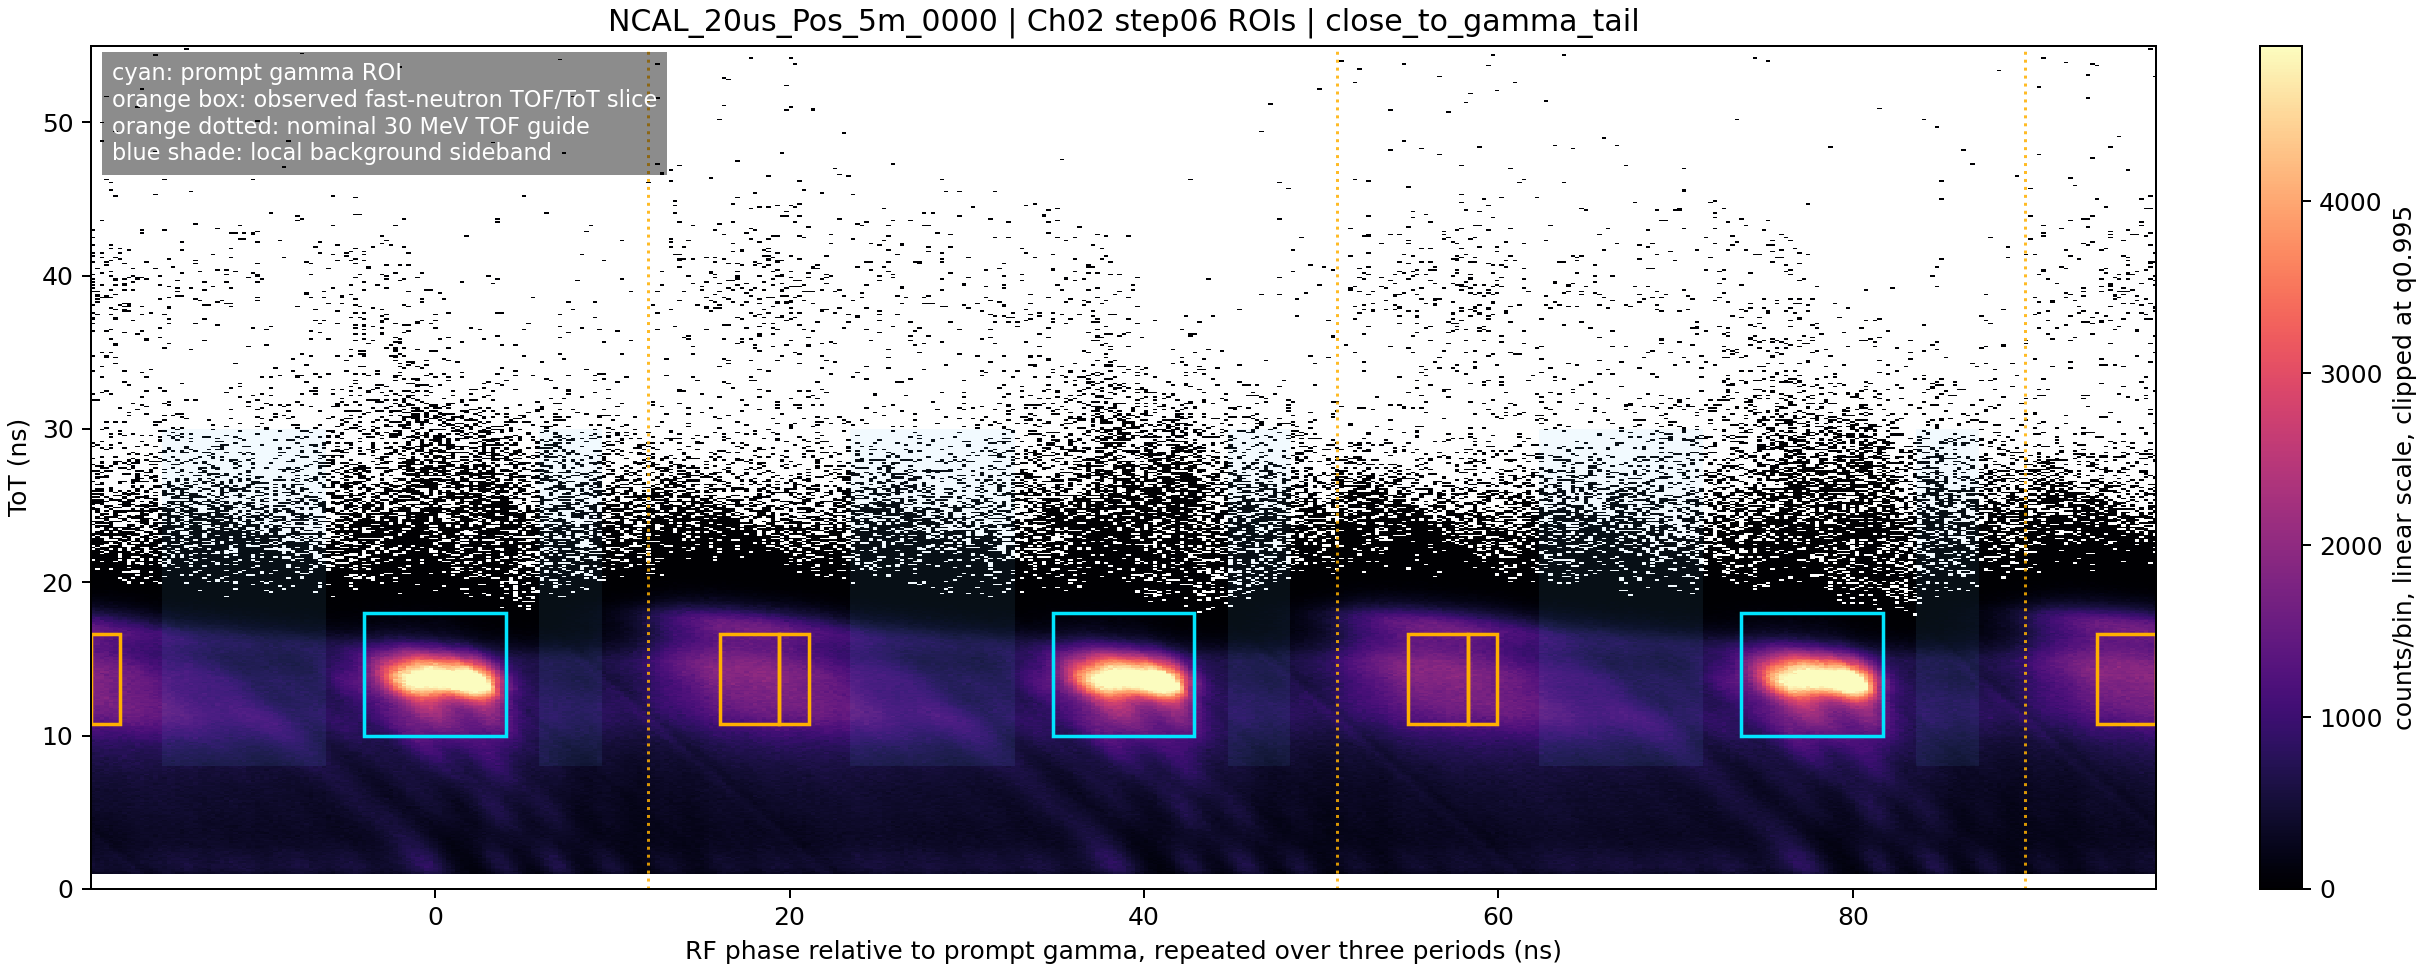
\includegraphics[width=0.96\textwidth]{../../Dogma_Analysis/Results/Position Runs/Gamma_Neutron_Components/overlays/NCAL_20us_Pos_5m_0000_ch02_step06_rois.png}

\vspace{0.8em}

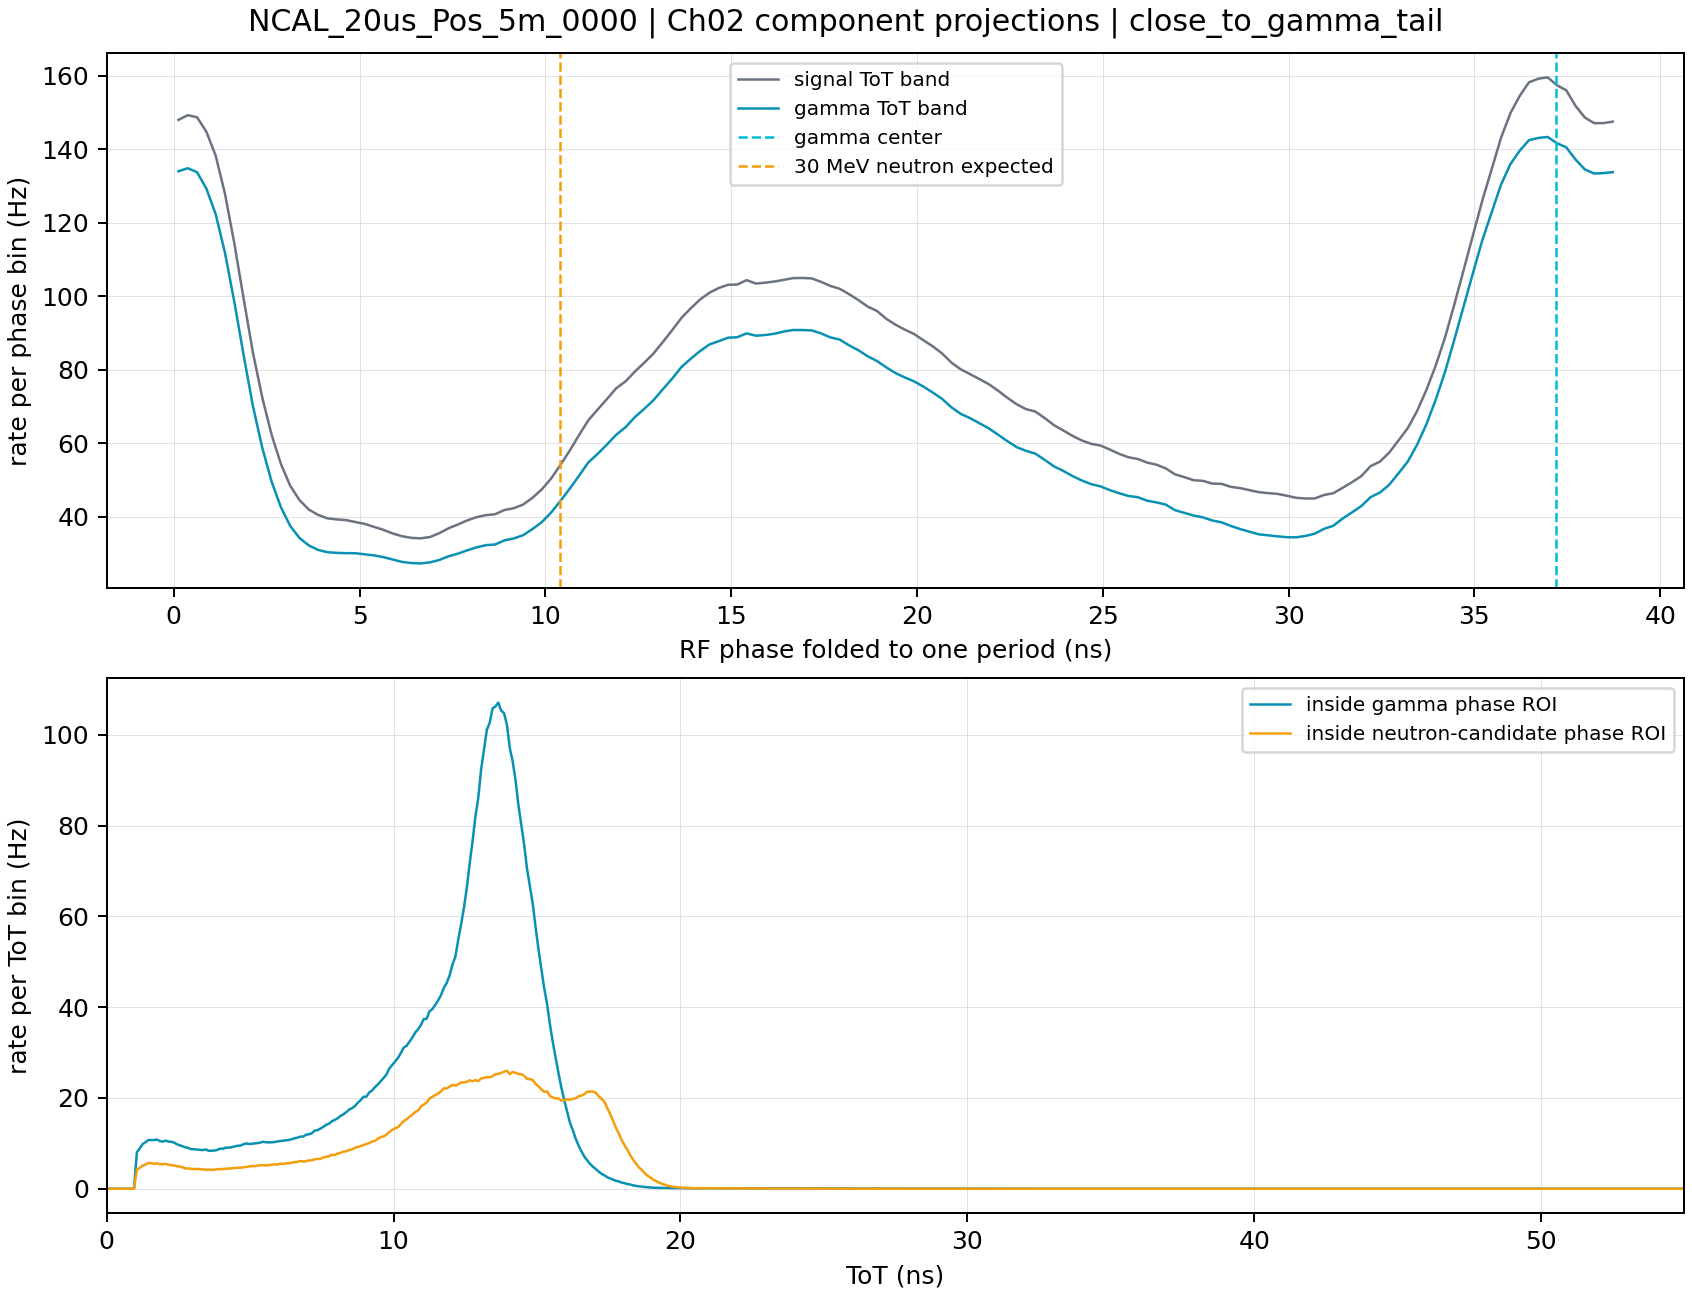
\includegraphics[width=0.94\textwidth]{../../Dogma_Analysis/Results/Position Runs/Gamma_Neutron_Components/projections/NCAL_20us_Pos_5m_0000_ch02_component_projections.png}
\caption{Representative step-06 gamma--neutron component diagnostics for the \SI{5.0}{m} run. Top: the phase--ToT overlay shows the prompt-gamma ROI, the nominal \SI{30}{MeV} TOF guide, the observed fast-neutron candidate slice, and the local background sidebands. Bottom: the one-dimensional phase and ToT projections show why the extracted neutron quantity is treated as a constrained fast-neutron slice rather than as the total neutron population.}
\label{fig:step06-roi-projections}
\end{figure}

\subsection{Prompt-gamma reference construction}

The practical challenge in the position scan is not only to identify a gamma-like island, but to anchor every run to a prompt-gamma reference that remains usable when the neutron population is converted into a time-of-flight scale. In overlap configurations the broad neutron-related structure can distort the prompt profile, so a reference extracted directly from a broad phase gate or from a leading-edge CFD construction is not sufficiently stable across all detector positions.

The first dedicated diagnostic is \path{step07_phase_rate_slice_diagnostics.py}. It collapses selected ToT intervals to one RF period, converts them to rates, and identifies delayed excess intervals relative to a robust off-prompt baseline. This is a selection-design diagnostic rather than a final physics extractor, but it provides an auditable one-dimensional check that the delayed structure is already present before one commits to specific two-dimensional boxes. Figure~\ref{fig:step07-phase-rate-slices} shows the representative \SI{5.0}{m} case used for this purpose.

\begin{figure}[htbp]
\centering
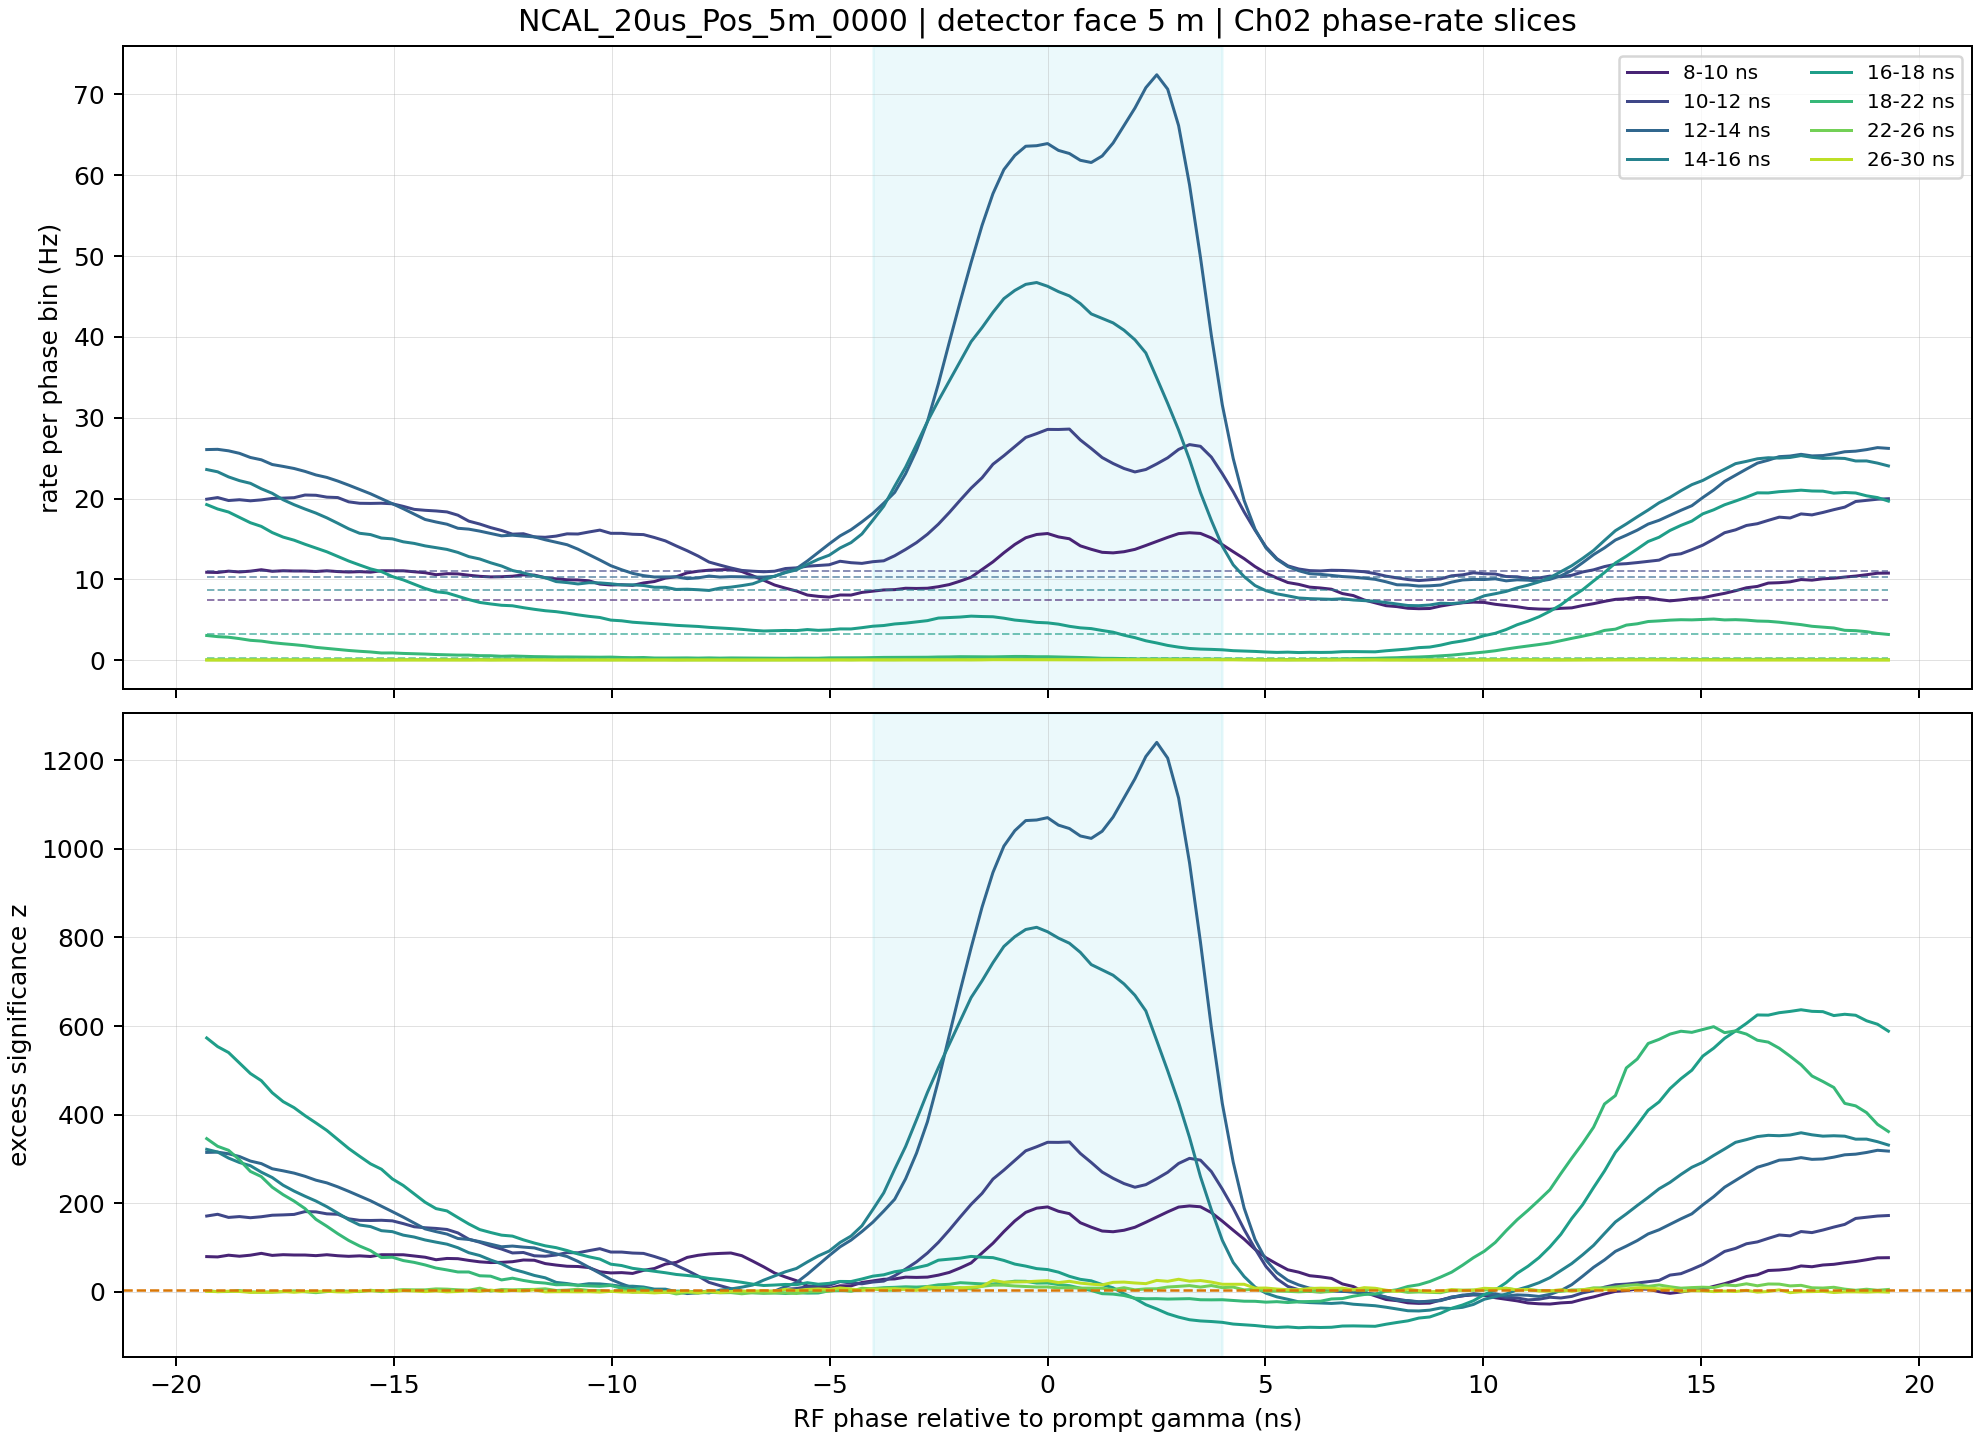
\includegraphics[width=0.96\textwidth]{../../Dogma_Analysis/Results/Position Runs/Phase_Rate_Slice_Diagnostics_5m/NCAL_20us_Pos_5m_0000_ch02_phase_rate_slices.png}
\caption{Representative step-07 one-period phase-rate diagnostics for the separated \SI{5.0}{m} case. The prompt-gamma band is centered at phase zero, and the delayed excess structure is inspected slice by slice in ToT before two-dimensional signal and background regions are finalized.}
\label{fig:step07-phase-rate-slices}
\end{figure}

The second stage is \path{step08_fit_gamma_tot_peak.py}, which fits the sharp channel-2 prompt-gamma ToT feature in the fixed interval \SIrange{12.5}{15.0}{ns} with a Gaussian plus constant background. Across the completed position runs, the fitted center remains tightly clustered, \(\mu_{\gamma}=\SIrange{13.580}{13.665}{ns}\), while the statistical fit uncertainty stays small, \(\sigma_{\mu}\approx\SIrange{0.0072}{0.0109}{ns}\). In the present workflow these fit errors are used as a centering precision for the prompt-gamma gate. They are not treated as a complete uncertainty budget for the full ToT distribution, because the broader spectrum is not exhaustively described by a single Gaussian plus constant term.

\begin{figure}[htbp]
\centering
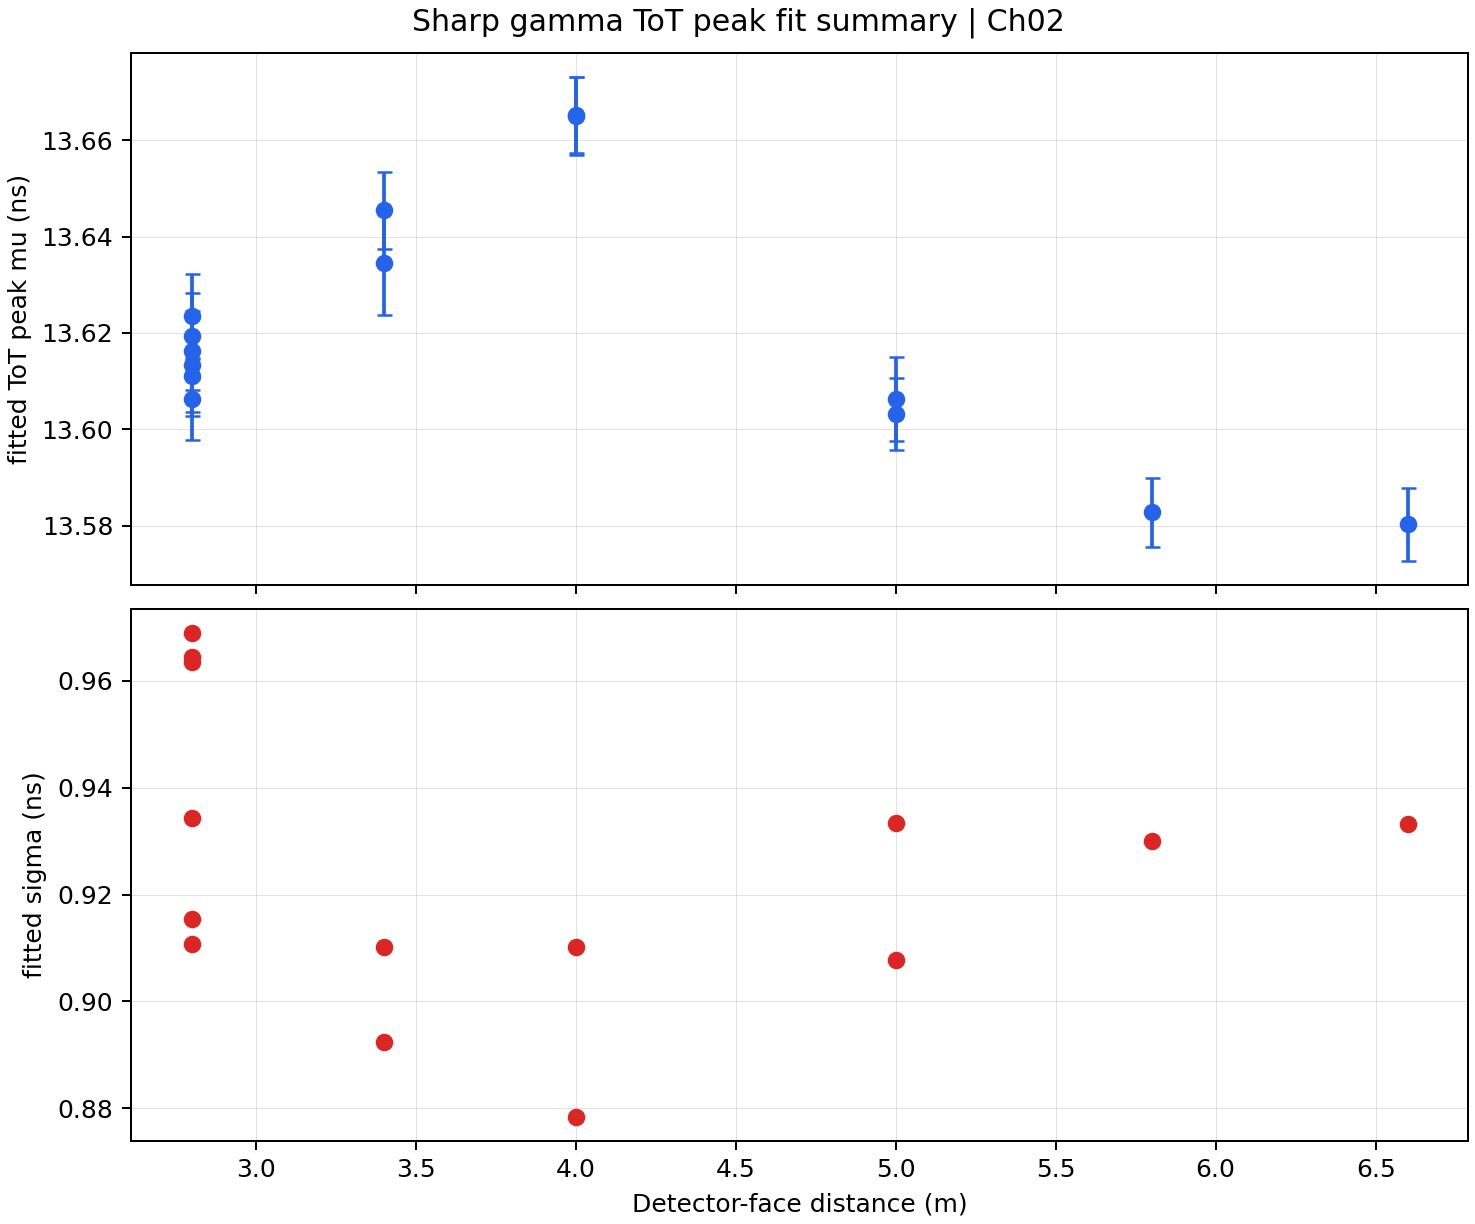
\includegraphics[width=0.80\textwidth]{../../Dogma_Analysis/Results/Position Runs/Gamma_TOT_Peak_Fits/gamma_tot_peak_fit_summary.png}
\caption{Summary of the step-08 narrow prompt-gamma ToT fits for channel~2. The fitted peak center remains stable across the completed position-scan runs, which justifies using \(\mu_{\gamma}\) as the run-by-run centering proxy for the prompt-gamma gate. The quoted fit errors are statistical under the chosen local model and should not be interpreted as the full systematic uncertainty of the pulse-width distribution.}
\label{fig:step08-gamma-tot-summary}
\end{figure}

After the prompt-gamma ToT gate has been centered on \(\mu_{\gamma}\), the final phase anchor is not taken from a single raw histogram bin. Instead, the cut-band one-period phase profile \(r_{\mathrm{cut}}(\phi)\) is formed and a local quadratic model
\begin{equation}
q(\phi) = a\phi^2 + b\phi + c
\end{equation}
is fitted in a narrow neighborhood around the cut-band maximum. The selected prompt-gamma reference is the fitted vertex,
\begin{equation}
\phi_{\mathrm{ref}} = -\frac{b}{2a},
\end{equation}
with fallback to the seed maximum if the fitted curvature is not concave or if the vertex escapes the local fit window. This choice keeps the reference tied to the prompt peak while reducing one-bin jumps that can appear when the cut-band top is slightly split or asymmetric.

Two further diagnostics are then used. Step~09 varies the prompt-gamma ToT half-width around \(\mu_{\gamma}\) and rebuilds the anchor to test window sensitivity. Step~10 compares the resulting local-fit reference against raw-maximum and CFD-style alternatives. In the present working document these studies are treated as systematic-control diagnostics rather than as a substitute for a full publication-level uncertainty budget. The prudent scientific statement is therefore that the current prompt-gamma anchor is designed to be sub-bin stable and auditable, while the final uncertainty budget should also absorb gate-width choice, binning dependence, and overlap-dependent background structure.

\subsection{Current production status}

In its current form, the DOGMA chain should be regarded as the robust production baseline for the commissioning data set. It already incorporates the main solutions required by the present beamtime analysis: pulse-level cleaning, explicit \texttt{ch0} auditing, consistent trigger- and channel-0-referenced observables, RF-folding diagnostics, within-run phase segmentation, first-pass background estimation, component studies for the position scan, and a multi-stage prompt-gamma anchoring strategy.

At the same time, not every diagnostic should yet be read as a finalized physics result. In particular, direct neutron numbers extracted from overlap runs remain constrained ROI measurements rather than total neutron yields, and the prompt-gamma anchor studies are best interpreted as the current methodological baseline for a later fully synchronized remote production. This distinction between validated workflow and finalized physics observable is essential if the document is to remain both reproducible and academically honest.

\section{CAEN analysis}

The CAEN-based path is presently an analysis-adjacent commissioning branch rather than the synchronized physics baseline of the beamtime. In practice, the DT5725S plus \textit{CoMPASS} chain has been used to verify detector response, threshold behavior, rate stability, and the general readiness of the front-end electronics. Those studies are scientifically useful because they constrain whether later timing or pulse-shape observables can be trusted, but they do not yet form a curated repository-scale result chain analogous to the DOGMA cleaned-data workflow.

Accordingly, the current CAEN analysis should be described conservatively as a validated instrumentation and signal-quality study. A fuller CAEN analysis section would eventually need curated list-mode or waveform datasets, explicit calibration logic, dead-time treatment, and figure-level outputs that can be cross-compared with the DOGMA observables on equal footing.

\section{Oscilloscope-supported analysis}

Oscilloscope measurements are not the primary archival data source of the present campaign, but they remain essential as a support-analysis instrument. Direct waveform inspection is the fastest way to identify baseline motion, overshoot, reflections, saturation, polarity mistakes, PMT light leaks, or cable problems before those effects appear indirectly in digitized timing or ToT observables. In that sense, oscilloscope work belongs to the analysis chapter because it constrains the physical interpretation of later digital observables even when the oscilloscope traces themselves are not the final published dataset.

At the present stage, these oscilloscope-supported studies are mainly qualitative or semi-quantitative diagnostics. They define the boundary conditions under which the digitized data can be trusted, but they do not yet constitute a stand-alone repository-scale analysis branch with synchronized result figures comparable to the DOGMA chain.

\section{DiRICH analysis context}

The DiRICH-based readout path remains scientifically relevant as a comparison branch because earlier NCAL work used that chain and because comparative readout studies are important for detector-development decisions. The key comparison questions are not only hardware oriented. They also concern timing-reference stability, data integrity, pulse-width behavior, analysis overhead, and the extent to which later particle-identification observables can be extracted reproducibly.

At present, however, the synchronized analysis products curated in this repository are DOGMA based. The DiRICH section is therefore intentionally brief and should be read as methodological context rather than as a fully developed results section. A mature DiRICH analysis treatment would require curated aligned datasets and direct observable-level comparisons against the DOGMA baseline.